\documentclass[12pt,a4paper]{elsarticle}
\usepackage[margin=0.5in]{geometry}
\usepackage{amssymb}
\usepackage{subfig}
\usepackage{float}
%\usepackage{subfigure}
\usepackage{hyperref}
\hypersetup{colorlinks=true,linkcolor=blue}
\usepackage{amsmath}
\usepackage{tikz}
\usepackage{lipsum}
\usetikzlibrary{arrows.meta}
\usetikzlibrary{arrows}
\usepackage{pstricks}
\usetikzlibrary{fadings}
%\usepackage{graphicx}
% \usepackage[nodots,nocompress]{numcompress}
 	\definecolor{ig}{rgb}{0.07, 0.53, 0.03}
 	\definecolor{cd}{rgb}{0.89, 0.0, 0.13}


 	\tikzset{
    geo/.pic = {
         %back square
% \draw [fill=orange] (-1,-1,1) rectangle (1,-1,1);
\draw[dashed,thick] (0,0,0) -- (1.5,0,0);
\draw[solid,thick] (1.5,0,0) -- (1.5,1,0);
\draw[solid,thick] (1.5,1,0) -- (0,1,0);
\draw[dashed,thick] (0,1,0) -- (0,0,0);

 %front square
% \draw [fill=orange] (-1,-1,1) rectangle (1,-1,1);
\draw[solid,thick] (0,0,3) -- (1.5,0,3);
\draw[solid,thick] (1.5,0,3) -- (1.5,1,3);
\draw[solid,thick] (1.5,1,3) -- (0,1,3);
\draw[solid,thick] (0,1,3) -- (0,0,3);

\draw[solid,thick] (0,1,0) -- (0,1,3);
\draw[solid,thick] (1.5,1,0) -- (1.5,1,3);
\draw[dashed,thick] (0,0,0) -- (0,0,3);
\draw[solid,thick] (1.5,0,0) -- (1.5,0,3);

\path[draw=black,solid,line width=0.1mm,preaction={-triangle 45,black,thin,draw,shorten >=-1mm}](0,0,0) -- (0.15,0,0);	%node x
\draw (0.2,0.05,0)node[gray]{$\mathbf{x}$};
\path[draw=black,solid,line width=0.1mm,preaction={-triangle 45,black,thin,draw,shorten >=-1mm}](0,0,0) -- (0,0.15,0);	%node y
\draw (-0.05,0.15,0)node[gray]{$\mathbf{y}$};
\path[draw=black,solid,line width=0.1mm,preaction={-triangle 45,black,thin,draw,shorten >=-1mm}](0,0,0) -- (0,0,0.15);	%node z
\draw (-0.05,0,0.2)node[gray]{$\mathbf{z}$};

\path[draw=black,solid,line width=0.1mm,preaction={-triangle 45,black,thin,draw,shorten >=-1mm}](1,-0.1,0) -- (1.3,-0.1,0);	%node E
\draw (1.15,-0.18,0)node[black]{$E$};
\path[draw=black,solid,line width=0.1mm,preaction={-triangle 45,black,thin,draw,shorten >=-1mm}](0.6,1.2,3) -- (0.3,1.2,3);	%node W
\draw (0.45,1.28,3)node[black]{$W$};
\path[draw=black,solid,line width=0.1mm,preaction={-triangle 45,black,thin,draw,shorten >=-1mm}](-0.05,0.4,0) -- (-0.05,0.7,0);	%node N
\draw (-0.12,0.55,0)node[black]{$N$};
\path[draw=black,solid,line width=0.1mm,preaction={-triangle 45,black,thin,draw,shorten >=-1mm}](1.6,0.7,3) -- (1.6,0.4,3);	%node S
\draw (1.65,0.55,3)node[black]{$S$};
\path[draw=black,solid,line width=0.1mm,preaction={-triangle 45,black,thin,draw,shorten >=-1mm}](0.9,0.5,0) -- (1.1,0.7,0);	%node B
\draw (0.95,0.65,0)node[black]{$B$};
\path[draw=black,solid,line width=0.2mm,preaction={-triangle 45,black,thin,draw,shorten >=-1mm}] (0.9,0.7,4) -- (0.7,0.5,4);	%node F
\draw (0.85,0.55,4)node[black]{$F$};
    }
}

\tikzset{
    lat/.pic = {

    \draw (-0.05,0.15,0)node[]{$\mathbf{0}$};

%nodes
\path[draw=black,solid,line width=0.2mm,fill=red,preaction={-triangle 45,black,thin,draw,shorten >=-1mm}](0,0,0) -- (1,0,0);	%node 1
\draw (1.1,-0.05,0)node[]{$\mathbf{1}$};
\path[draw=black,solid,line width=0.2mm,fill=black,preaction={-triangle 45,black,thin,draw,shorten >=-1mm}](0,0,0) -- (-1,0,0);	%node 2
\draw (-1.1,-0.05,0)node[]{$\mathbf{2}$};
\path[draw=black,solid,line width=0.2mm,fill=black,preaction={-triangle 45,black,thin,draw,shorten >=-1mm}](0,0,0) -- (0,1,0);	%node 3
\draw (0,1.1,0)node[]{$\mathbf{3}$};
\path[draw=black,solid,line width=0.2mm,fill=black,preaction={-triangle 45,black,thin,draw,shorten >=-1mm}](0,0,0) -- (0,-1,0);	%node 4
\draw (0,-1.1,0)node[]{$\mathbf{4}$};
\path[draw=black,solid,line width=0.2mm,fill=black,preaction={-triangle 45,black,thin,draw,shorten >=-1mm}](0,0,0) -- (0,0,1);	%node 5
\draw (-0.1,0.1,1)node[]{$\mathbf{5}$};
\path[draw=black,solid,line width=0.2mm,fill=black,preaction={-triangle 45,black,thin,draw,shorten >=-1mm}](0,0,0) -- (0,0,-1);	%node 6
\draw (-0.1,0.1,-1)node[]{$\mathbf{6}$};

\path[draw=ig,solid,line width=0.2mm,preaction={-triangle 45,ig,thin,draw,shorten >=-1mm}](0,0,0) -- (1,1.05,0.2);	%node 7
\draw (1.05,1.2,0.2)node[ig]{$\mathbf{7}$};
\path[draw=ig,solid,line width=0.2mm,preaction={-triangle 45,ig,thin,draw,shorten >=-1mm}](0,0,0) -- (-1,-1.05,-0.2);	%node 8
\draw (-1,-1.2,-0.2)node[ig]{$\mathbf{8}$};
\path[draw=ig,solid,line width=0.2mm,preaction={-triangle 45,ig,thin,draw,shorten >=-1mm}](0,0,0) -- (1,-1,0);	%node 13
\draw (1.15,-1,0)node[ig]{$\mathbf{13}$};
\path[draw=ig,solid,line width=0.2mm,preaction={-triangle 45,ig,thin,draw,shorten >=-1mm}](0,0,0) -- (-1,1,0);	%node 14
\draw (-1.2,1,0)node[ig]{$\mathbf{14}$};



\path[draw=red,solid,line width=0.2mm,preaction={-triangle 45,red,thin,draw,shorten >=-1mm}](0,0,0) -- (1,0,1);	%node 9
\draw (1.1,-0.05,1)node[red]{$\mathbf{9}$};
\path[draw=red,solid,line width=0.2mm,preaction={-triangle 45,red,thin,draw,shorten >=-1mm}](0,0,0) -- (-1,0,-1);	%node 10
\draw (-1.2,0,-1)node[red]{$\mathbf{10}$};
\path[draw=red,solid,line width=0.2mm,preaction={-triangle 45,red,thin,draw,shorten >=-1mm}](0,0,0) -- (1,0,-1);	%node 15
\draw (1.1,0,-1)node[red]{$\mathbf{15}$};
\path[draw=red,solid,line width=0.2mm,preaction={-triangle 45,red,thin,draw,shorten >=-1mm}](0,0,0) -- (-1,0,1);	%node 16
\draw (-1.2,0,1)node[red]{$\mathbf{16}$};



\path[draw=blue,solid,line width=0.2mm,preaction={-triangle 45,blue,thin,draw,shorten >=-1mm}](0,0,0) -- (0,1,1);	%node 11
\draw (-0.1,1.1,1)node[blue]{$\mathbf{11}$};
\path[draw=blue,solid,line width=0.2mm,preaction={-triangle 45,blue,thin,draw,shorten >=-1mm}](0,0,0) -- (0,1,-1);	%node 17
\draw (0,1.1,-1)node[blue]{$\mathbf{17}$};
\path[draw=blue,solid,line width=0.2mm,preaction={-triangle 45,blue,thin,draw,shorten >=-1mm}](0,0,0) -- (0,-1,1);	%node 18
\draw (0,-1.1,1)node[blue]{$\mathbf{18}$};
\path[draw=blue,solid,line width=0.2mm,preaction={-triangle 45,blue, thin,draw,shorten >=-1mm}](0,0,0) -- (0,-1,-1);	%node 12
\draw (0.1,-1.1,-1)node[blue]{$\mathbf{12}$};

\draw[blue,fill=blue] (0,0,0)node[]{} circle(0.04cm);


%Front square
% \draw [fill=orange] (-1,-1,1) rectangle (1,-1,1);
\draw[solid,thick] (-1,-1,1) -- (1,-1,1);
\draw[solid,thick] (1,-1,1) -- (1,1,1);
\draw[solid,thick] (1,1,1) -- (-1,1,1);
\draw[solid,thick] (-1,1,1) -- (-1,-1,1);

%Back square
\draw[solid,thick] (-1,-1,-1) -- (1,-1,-1);
\draw[solid,thick] (1,-1,-1) -- (1,1,-1);
\draw[solid,thick] (1,1,-1) -- (-1,1,-1);
\draw[solid,thick] (-1,1,-1) -- (-1,-1,-1);

%Edges
\draw[solid,thick] (-1,-1,1) -- (-1,-1,-1); % bottem left
\draw[solid,thick] (1,-1,1) -- (1,-1,-1); % bottem right
\draw[solid,thick] (-1,1,-1) -- (-1,1,1);  % top left
\draw[solid,thick] (1,1,-1) -- (1,1,1);  % top right

%mid planes
%x=0 plane
\draw[blue,dashed, thin] (0,-1,1) -- (0,-1,-1);
\draw[blue,dashed, thin] (0,-1,-1) -- (0,1,-1);
\draw[blue,dashed, thin] (0,1,-1) -- (0,1,1);
\draw[blue,dashed, thin] (0,1,1) --(0,-1,1);
%y=0 planed
\draw[red,thin,dashed] (-1,0,1) -- (1,0,1);
\draw[red,thin,dashed] (1,0,1) -- (1,0,-1);
\draw[red,thin,dashed] (1,0,-1) --  (-1,0,-1);
\draw[red,thin,dashed] (-1,0,-1) -- (-1,0,1);
%z=0 plane
\draw[ig,thin,dashed] (-1,-1,0) -- (1,-1,0);
\draw[ig,thin,dashed] (1,-1,0) -- (1,1,0);
\draw[ig,thin,dashed] (1,1,0) -- (-1,1,0);
\draw[ig,thin,dashed] (-1,1,0) -- (-1,-1,0);

\path[draw=gray,solid,line width=0.2mm,preaction={-triangle 45,gray,thin,draw,shorten >=-1mm}](-1.1,-1.1,1.1) -- (-0.8,-1.1,1.1);	%node x
\draw (-0.7,-1.1,1.1)node[gray]{$\mathbf{x}$};
\path[draw=gray,solid,line width=0.2mm,preaction={-triangle 45,gray,thin,draw,shorten >=-1mm}](-1.1,-1.1,1.1) -- (-1.1,-0.8,1.1);	%node y
\draw (-1.1,-0.7,1.1)node[gray]{$\mathbf{y}$};
\path[draw=gray,solid,line width=0.2mm,preaction={-triangle 45,gray,thin,draw,shorten >=-1mm}](-1.1,-1.1,1.1) -- (-1.1,-1.1,1.5);	%node z
\draw (-1.1,-1.1,1.65)node[gray]{$\mathbf{z}$};

    }
}


\begin{document}
\begin{figure}[t] %Needs to be modified!!!!!!!!!!!!!!!!
  \centering
  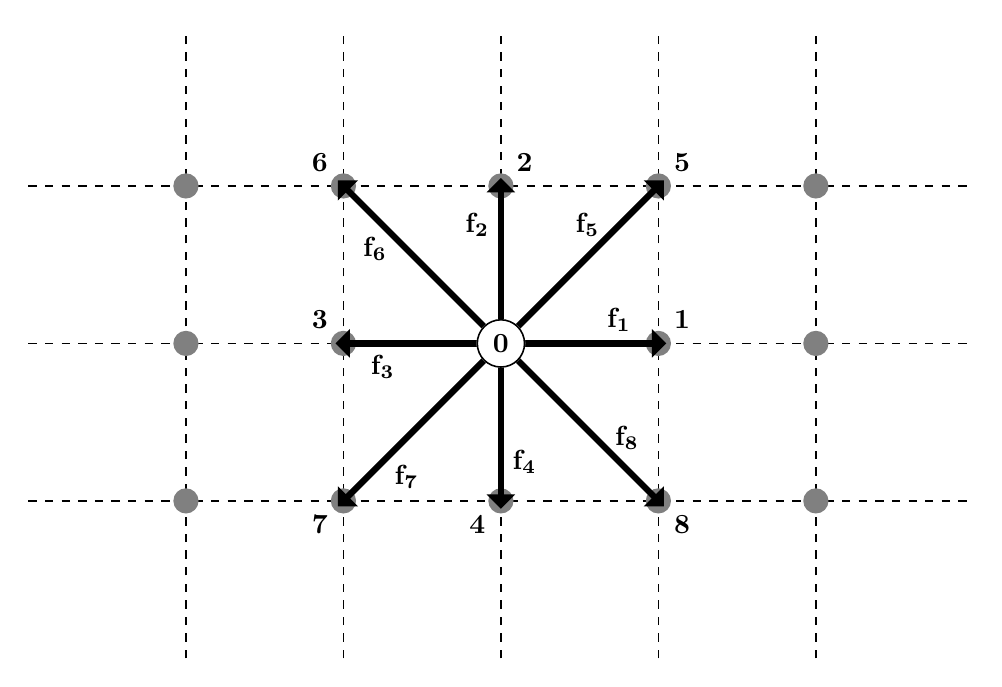
\begin{tikzpicture}[line width=0.2mm]

    %\draw [dashed,line width=0.5mm] (0,0) rectangle(12,8);
    \draw[dashed] (0,2) -- (12,2);
    \draw[dashed] (0,4) -- (12,4);
    \draw[dashed] (0,6) -- (12,6);
    \draw[dashed] (2,0) -- (2,8);
    \draw[dashed] (4,0) -- (4,8);
    \draw[dashed] (6,0) -- (6,8);
    \draw[dashed] (8,0) -- (8,8);
    \draw[dashed] (10,0) -- (10,8);

    \draw[gray,fill=gray] (2,2)node[]{} circle(0.15cm);
    \draw[gray,fill=gray] (4,2)node[]{} circle(0.15cm);
    \draw[gray,fill=gray] (6,2)node[]{} circle(0.15cm);
    \draw[gray,fill=gray] (8,2)node[]{} circle(0.15cm);
    \draw[gray,fill=gray] (10,2)node[]{} circle(0.15cm);

    \draw[gray,fill=gray] (2,4)node[]{} circle(0.15cm);
    \draw[gray,fill=gray] (4,4)node[]{} circle(0.15cm);
    %\draw[black,fill=black] (6,4)node[]{} circle(0.15cm);
    \draw[gray,fill=gray] (8,4)node[]{} circle(0.15cm);
    \draw[gray,fill=gray] (10,4)node[]{} circle(0.15cm);

    \draw[gray,fill=gray] (2,6)node[]{} circle(0.15cm);
    \draw[gray,fill=gray] (4,6)node[]{} circle(0.15cm);
    \draw[gray,fill=gray] (6,6)node[]{} circle(0.15cm);
    \draw[gray,fill=gray] (8,6)node[]{} circle(0.15cm);
    \draw[gray,fill=gray] (10,6)node[]{} circle(0.15cm);

    \path[draw=black,solid,line width=0.8mm,fill=black,preaction={-triangle 90,thick,draw,shorten >=-1mm}](6,4) -- (8,4);
    \path[draw=black,solid,line width=0.8mm,fill=black,preaction={-triangle 90,thick,draw,shorten >=-1mm}](6,4) -- (4,4);
    \path[draw=black,solid,line width=0.8mm,fill=black,preaction={-triangle 90,thick,draw,shorten >=-1mm}](6,4) -- (6,6);
    \path[draw=black,solid,line width=0.8mm,fill=black,preaction={-triangle 90,thick,draw,shorten >=-1mm}](6,4) -- (6,2);
    \path[draw=black,solid,line width=0.8mm,fill=black,preaction={-triangle 90,thick,draw,shorten >=-1mm}](6,4) -- (8,6);
    \path[draw=black,solid,line width=0.8mm,fill=black,preaction={-triangle 90,thick,draw,shorten >=-1mm}](6,4) -- (4,6);
    \path[draw=black,solid,line width=0.8mm,fill=black,preaction={-triangle 90,thick,draw,shorten >=-1mm}](6,4) -- (4,2);
    \path[draw=black,solid,line width=0.8mm,fill=black,preaction={-triangle 90,thick,draw,shorten >=-1mm}](6,4) -- (8,2);

    \draw[white,fill=white] (6,4)node[]{} circle(0.3cm);
    \draw (6,4) circle [radius=0.3] node {$\mathbf{0}$};
    %\draw (5.8,4.6)node[]{$\mathbf{0}$};
    \draw (8.3,4.3)node[]{$\mathbf{1}$};
    \draw (6.3,6.3)node[]{$\mathbf{2}$};
    \draw (3.7,4.3)node[]{$\mathbf{3}$};
    \draw (5.7,1.7)node[]{$\mathbf{4}$};
    \draw (8.3,6.3)node[]{$\mathbf{5}$};
    \draw (3.7,6.3)node[]{$\mathbf{6}$};
    \draw (3.7,1.7)node[]{$\mathbf{7}$};
    \draw (8.3,1.7)node[]{$\mathbf{8}$};

    \draw (7.5,4.3)node[]{$\mathbf{f_1}$};
    \draw (5.7,5.5)node[]{$\mathbf{f_2}$};
    \draw (4.5,3.7)node[]{$\mathbf{f_3}$};
    \draw (6.3,2.5)node[]{$\mathbf{f_4}$};
    \draw (7.1,5.5)node[]{$\mathbf{f_5}$};
    \draw (4.4,5.2)node[]{$\mathbf{f_6}$};
    \draw (4.8,2.3)node[]{$\mathbf{f_7}$};
    \draw (7.6,2.8)node[]{$\mathbf{f_8}$};
  \end{tikzpicture}
  \caption{Lattice directions and corresponding velocities for D2Q9 model}
  \label{fig:D2Q9 lattice model}
\end{figure}

\begin{center}
  \Large{\textbf{Corners}}
\end{center}
1. South-West-Back
\begin{figure}[!h]
  \centering

  \subfloat[]{
    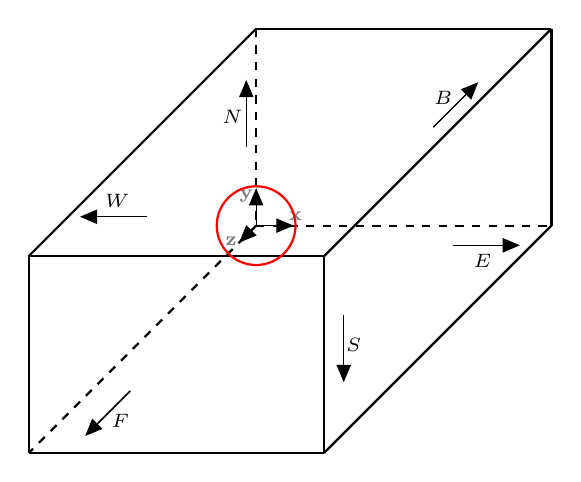
\begin{tikzpicture}[]
      \path pic[font=\scriptsize,scale=2.50]{geo};
      \draw[red,thick] (0,0,0) circle (0.5);
    \end{tikzpicture}
  }
  \subfloat[]{
    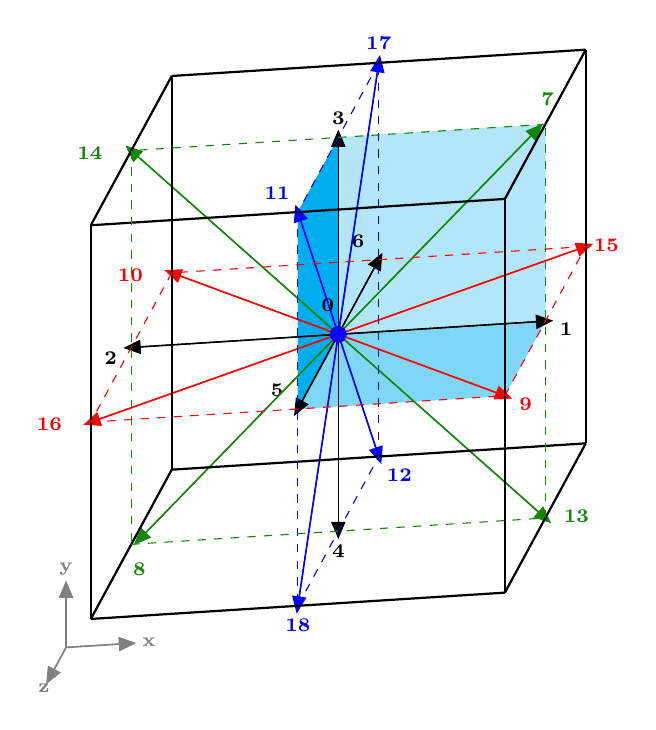
\begin{tikzpicture}[font=\scriptsize,scale=2.50,rotate around y=10,rotate around y=0]
      \fill[cyan!50] (1,1,1) -- (0,1,1) -- (0,0,1) -- (1,0,1) -- cycle; %  4.east-north-front
      \fill[cyan!50] (1,1,1) -- (0,1,1) -- (0,1,0) -- (1,1,0) -- cycle;
      \fill[cyan!50] (1,1,1) -- (1,1,0) -- (1,0,0) -- (1,0,1) -- cycle;

      \fill[cyan!50] (1,0,1) -- (0,0,1) -- (0,0,0) -- (1,0,0) -- cycle;
      \fill[cyan!30] (1,1,0) -- (0,1,0) -- (0,0, 0) -- (1,0,0) -- cycle;
      \fill[cyan] (0,1,1) -- (0,1,0) -- (0,0,0) -- (0,0,1) -- cycle;

      \path pic[font=\scriptsize,scale=2.50]{lat};
    \end{tikzpicture}
  }
  \caption{I=\{ 0,2,4,6,8,10,12\} and O=\{ 0,1,3,5,7,9,11\}}
\end{figure}

2. South-West-front
\begin{figure}[!h]
  \centering

  \subfloat[]{
    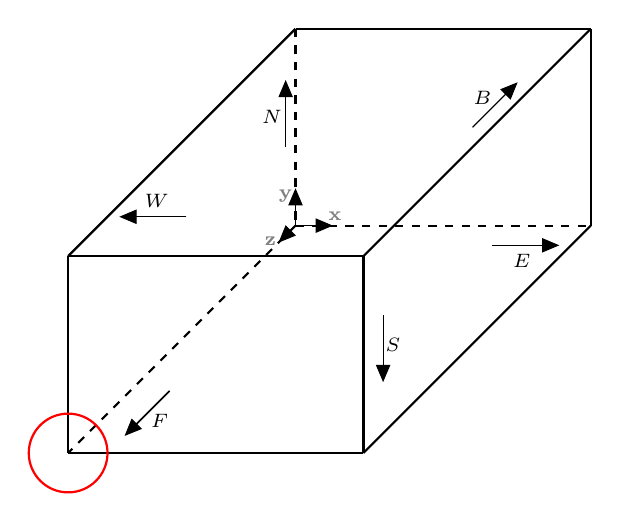
\begin{tikzpicture}[]
      \path pic[font=\scriptsize,scale=2.50]{geo};
      \draw[red,thick,scale=2.50] (0,0,3) circle (0.2);
    \end{tikzpicture}
  }
  \subfloat[]{
    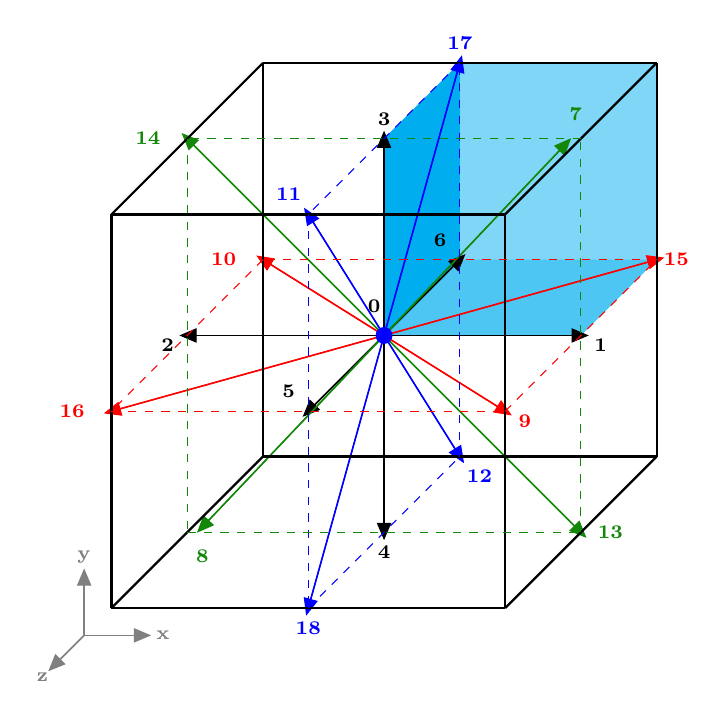
\begin{tikzpicture}[font=\scriptsize,scale=2.50,rotate around y=0,rotate around y=0]
      \fill[cyan!50] (1,1,-1) -- (0,1,-1) -- (0,0,-1) -- (1,0,-1) -- cycle; %  8. east-north-back
      \fill[cyan!50] (1,1,-1) -- (0,1,-1) -- (0,1,0) -- (1,1,0) -- cycle;
      \fill[cyan!50] (1,1,-1) -- (1,1,0) -- (1,0,0) -- (1,0,-1) -- cycle;

      \fill[cyan!50] (1,1,0) -- (0,1,0) -- (0,0, 0) -- (1,0,0) -- cycle;
      \fill[cyan] (0,1,-1) -- (0,1,0) -- (0,0,0) -- (0,0,-1) -- cycle;
      \fill[cyan!70] (1,0,-1) -- (0,0,-1) -- (0,0,0) -- (1,0,0) -- cycle;

      \path pic[font=\scriptsize,scale=2.50]{lat};
    \end{tikzpicture}
  }
  \caption{I=\{ 0,2,4,5,8,16,18\} and O=\{ 0,1,3,6,7,15,17\}}
\end{figure}

3. North-West-back
\begin{figure}[H]
  \centering

  \subfloat[]{
    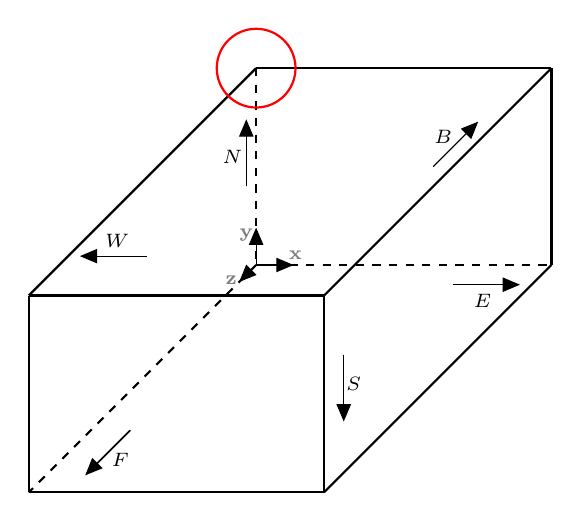
\begin{tikzpicture}[]
      \path pic[font=\scriptsize,scale=2.50]{geo};
      \draw[red,thick,scale=2.50] (0,1,0) circle (0.2);
    \end{tikzpicture}
  }
  \subfloat[]{
    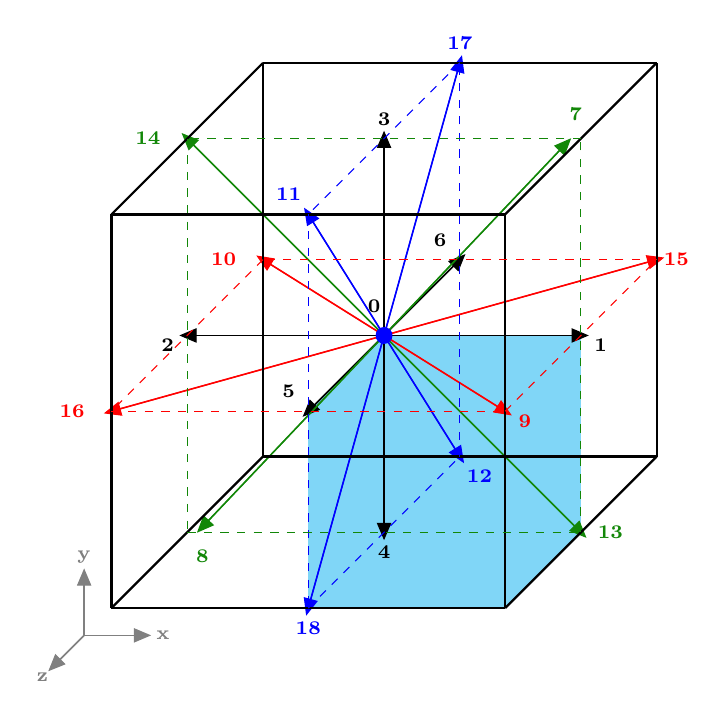
\begin{tikzpicture}[font=\scriptsize,scale=2.50,rotate around y=0,rotate around y=0]
      \fill[cyan!50] (0,-1,1) -- (1,-1,1) -- (1,0,1) -- (0,0,1) -- cycle;% 2. east-south-front
      \fill[cyan!50] (1,-1,1) -- (1,-1,0) -- (1,0,0) -- (1,0,1) -- cycle;
      \fill[cyan!50] (0,-1,1) -- (1,-1,1) -- (1,-1,0) -- (0,-1,0) -- cycle;
      \fill[cyan!50] (1,0,1) -- (0,0,1) -- (0,0,0) -- (1,0,0) -- cycle;
      \fill[cyan!50] (0,-1,0) -- (1,-1,0) -- (1,0, 0) -- (0,0,0) -- cycle;
      \fill[cyan!50] (0,-1,1) -- (0,-1,0) -- (0,0,0) -- (0,0,1) -- cycle;

      \path pic[font=\scriptsize,scale=2.50]{lat};
    \end{tikzpicture}
  }
  \caption{I=\{ 0,2,3,6,10,14,17\} and O=\{ 0,1,4,5,9,13,18\}}
\end{figure}

4. North-West-front
\begin{figure}[H]
  \centering

  \subfloat[]{
    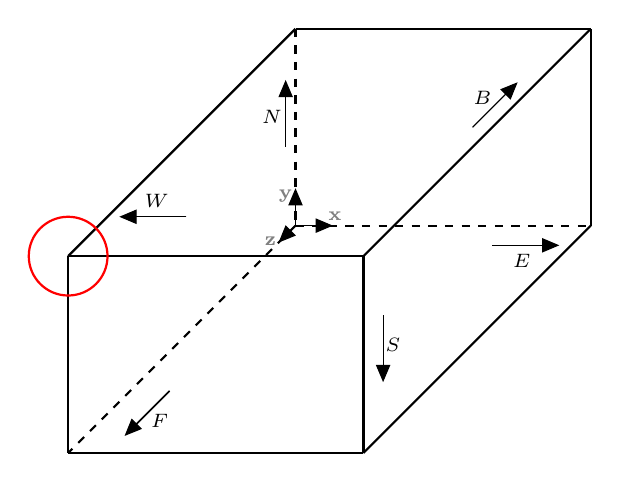
\begin{tikzpicture}[]
      \path pic[font=\scriptsize,scale=2.50]{geo};
      \draw[red,thick,scale=2.50] (0,1,3) circle (0.2);
    \end{tikzpicture}
  }
  \subfloat[]{
    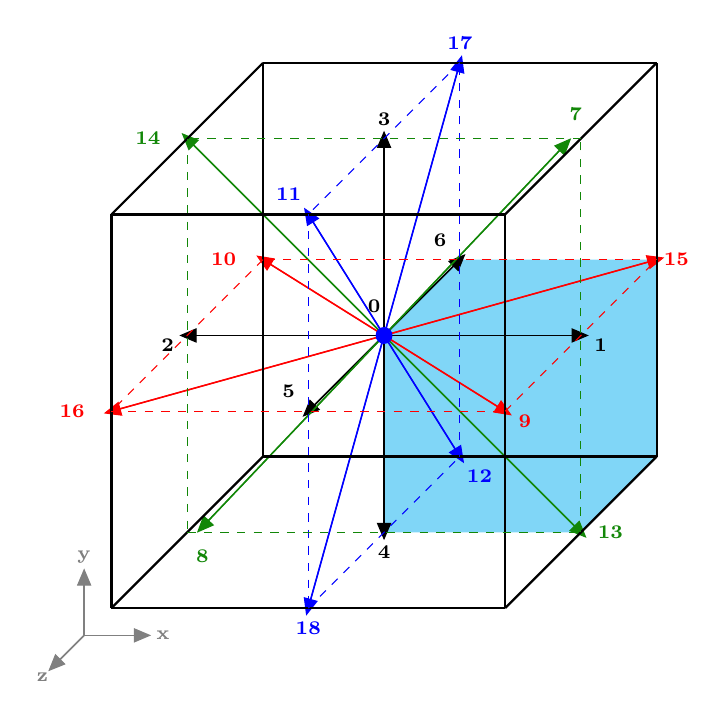
\begin{tikzpicture}[font=\scriptsize,scale=2.50,rotate around y=0,rotate around y=0]
      \fill[cyan!50] (1,-1,-1) -- (0,-1,-1) -- (0,0,-1) -- (1,0,-1) -- cycle; %  6.east-south-back
      \fill[cyan!50] (1,-1,-1) -- (0,-1,-1) -- (0,-1,0) -- (1,-1,0) -- cycle;
      \fill[cyan!50] (1,-1,-1) -- (1,-1,0) -- (1,0,0) -- (1,0,-1) -- cycle;
      \fill[cyan!50] (0,-1,-1) -- (0,-1,0) -- (0,0,0) -- (0,0,-1) -- cycle;
      \fill[cyan!50] (1,0,-1) -- (0,0,-1) -- (0,0,0) -- (1,0,0) -- cycle;
      \fill[cyan!50] (1,-1,0) -- (0,-1,0) -- (0,0, 0) -- (1,0,0) -- cycle;

      \path pic[font=\scriptsize,scale=2.50]{lat};
    \end{tikzpicture}
  }
  \caption{I=\{ 0,2,3,5,11,14,16\} and O=\{ 0,1,4,6,12,13,15\}}
\end{figure}

5. South-East-Back
\begin{figure}[H]
  \centering

  \subfloat[]{
    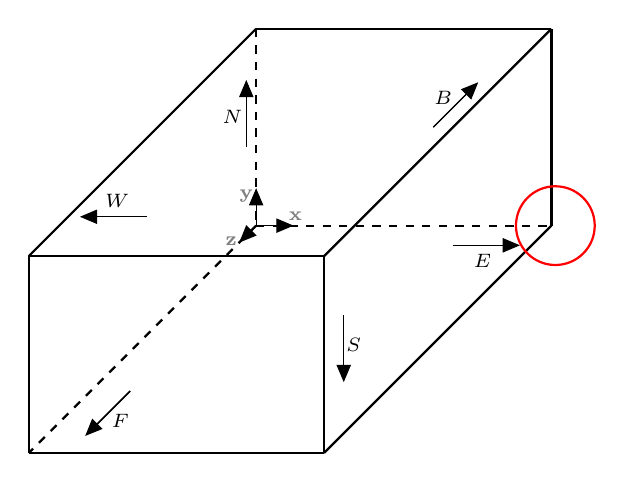
\begin{tikzpicture}[]
      \path pic[font=\scriptsize,scale=2.50]{geo};
      \draw[red,thick] (3.8,0,0) circle (0.5);
    \end{tikzpicture}
  }
  \subfloat[]{
    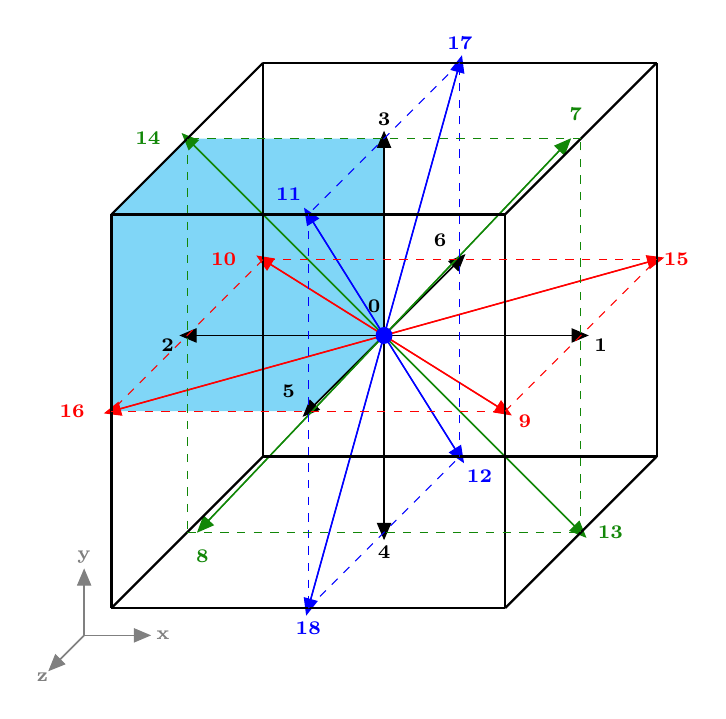
\begin{tikzpicture}[font=\scriptsize,scale=2.50,rotate around y=0,rotate around y=0]

      \fill[cyan!50] (-1,1,1) -- (0,1,1) -- (0,0,1) -- (-1,0,1) -- cycle; %  3.west-north-front
      \fill[cyan!50] (-1,1,1) -- (0,1,1) -- (0,1,0) -- (-1,1,0) -- cycle;
      \fill[cyan!50] (-1,1,1) -- (-1,1,0) -- (-1,0,0) -- (-1,0,1) -- cycle;
      \fill[cyan!50] (0,1,1) -- (0,1,0) -- (0,0,0) -- (0,0,1) -- cycle;
      \fill[cyan!50] (-1,0,1) -- (0,0,1) -- (0,0,0) -- (-1,0,0) -- cycle;
      \fill[cyan!50] (-1,1,0) -- (0,1,0) -- (0,0, 0) -- (-1,0,0) -- cycle;

      \path pic[font=\scriptsize,scale=2.50]{lat};
    \end{tikzpicture}
  }
  \caption{I=\{ 0,1,4,6,12,13,15\} and O=\{ 0,2,3,5,11,14,16\}}
\end{figure}

6. South-East-front
\begin{figure}[H]
  \centering

  \subfloat[]{
    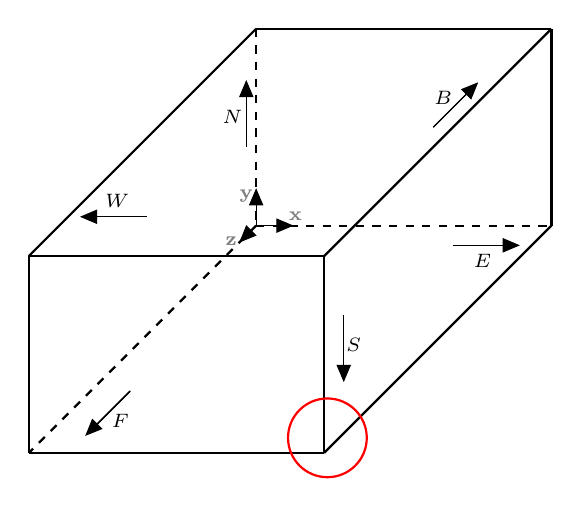
\begin{tikzpicture}[]
      \path pic[font=\scriptsize,scale=2.50]{geo};
      \draw[red,thick] (3.6,0,7) circle (0.5);
    \end{tikzpicture}
  }
  \subfloat[]{
    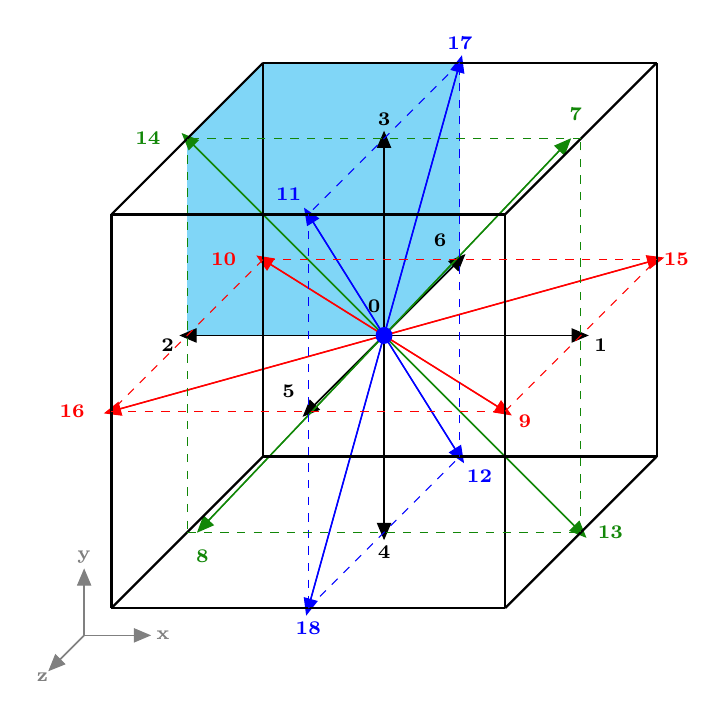
\begin{tikzpicture}[font=\scriptsize,scale=2.50,rotate around y=0,rotate around y=0]

      \fill[cyan!50] (-1,1,-1) -- (0,1,-1) -- (0,0,-1) -- (-1,0,-1) -- cycle; %  7.west-north-back
      \fill[cyan!50] (-1,1,-1) -- (0,1,-1) -- (0,1,0) -- (-1,1,0) -- cycle;
      \fill[cyan!50] (-1,1,-1) -- (-1,1,0) -- (-1,0,0) -- (-1,0,-1) -- cycle;
      \fill[cyan!50] (0,1,-1) -- (0,1,0) -- (0,0,0) -- (0,0,-1) -- cycle;
      \fill[cyan!50] (-1,0,-1) -- (0,0,-1) -- (0,0,0) -- (-1,0,0) -- cycle;
      \fill[cyan!50] (-1,1,0) -- (0,1,0) -- (0,0, 0) -- (-1,0,0) -- cycle;

      \path pic[font=\scriptsize,scale=2.50]{lat};
    \end{tikzpicture}
  }
  \caption{I=\{ 0,1,4,5,9,13,18\} and O=\{ 0,2,3,6,10,14,17\}}
\end{figure}

7. north-East-back
\begin{figure}[H]
  \centering

  \subfloat[]{
    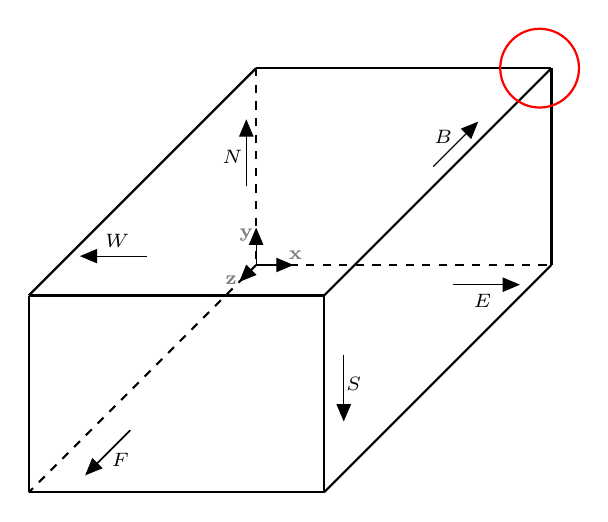
\begin{tikzpicture}[]
      \path pic[font=\scriptsize,scale=2.50]{geo};
      \draw[red,thick] (3.6,2.5,0) circle (0.5);
    \end{tikzpicture}
  }
  \subfloat[]{
    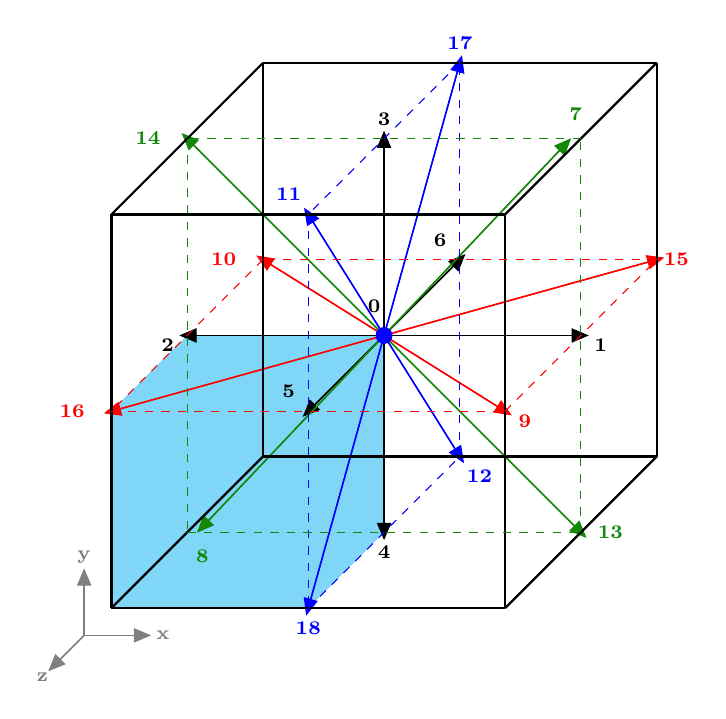
\begin{tikzpicture}[font=\scriptsize,scale=2.50,rotate around y=0,rotate around y=0]

      \fill[cyan!50] (-1,-1,1) -- (0,-1,1) -- (0,0,1) -- (-1,0,1) -- cycle; %  1.west-south-front
      \fill[cyan!50] (-1,-1,1) -- (0,-1,1) -- (0,-1,0) -- (-1,-1,0) -- cycle;
      \fill[cyan!50] (-1,-1,1) -- (-1,-1,0) -- (-1,0,0) -- (-1,0,1) -- cycle;
      \fill[cyan!50] (0,-1,1) -- (0,-1,0) -- (0,0,0) -- (0,0,1) -- cycle;
      \fill[cyan!50] (-1,0,1) -- (0,0,1) -- (0,0,0) -- (-1,0,0) -- cycle;
      \fill[cyan!50] (-1,-1,0) -- (0,-1,0) -- (0,0, 0) -- (-1,0,0) -- cycle;

      \path pic[font=\scriptsize,scale=2.50]{lat};
    \end{tikzpicture}
  }
  \caption{I=\{ 0,1,3,6,7,15,17\} and O=\{ 0,2,4,5,8,16,18\}}
\end{figure}

8. north-East-front
\begin{figure}[H]
  \centering

  \subfloat[]{
    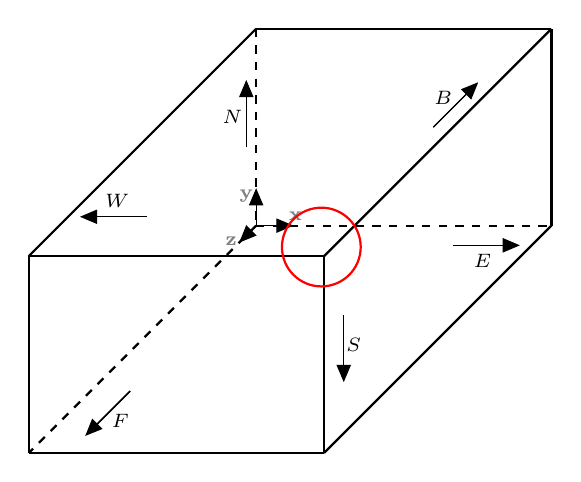
\begin{tikzpicture}[]
      \path pic[font=\scriptsize,scale=2.50]{geo};
      \draw[red,thick] (3.6,2.5,7.2) circle (0.5);
    \end{tikzpicture}
  }
  \subfloat[]{
    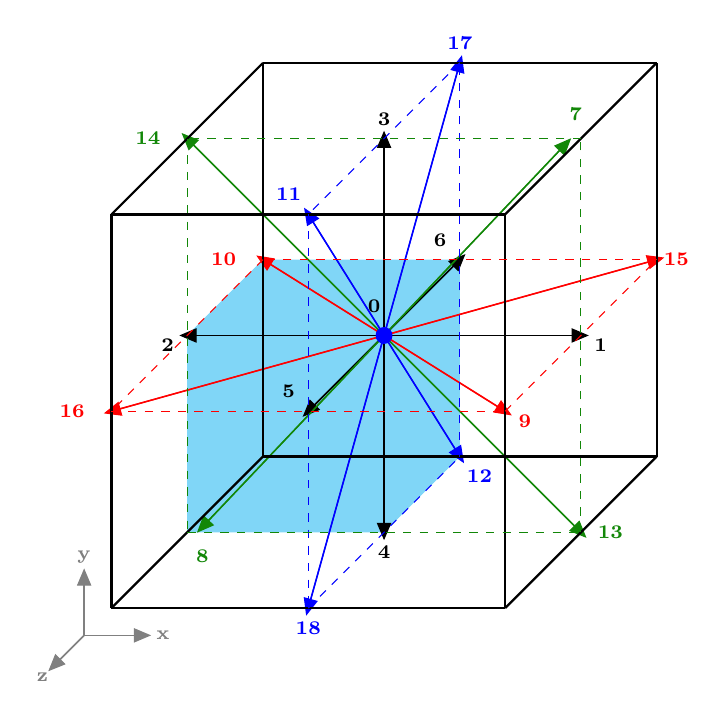
\begin{tikzpicture}[font=\scriptsize,scale=2.50,rotate around y=0,rotate around y=0]

      \fill[cyan!50] (-1,-1,-1) -- (0,-1,-1) -- (0,0,-1) -- (-1,0,-1) -- cycle; %  5. west-south-back
      \fill[cyan!50] (-1,-1,-1) -- (0,-1,-1) -- (0,-1,0) -- (-1,-1,0) -- cycle;
      \fill[cyan!50] (-1,-1,-1) -- (-1,-1,0) -- (-1,0,0) -- (-1,0,-1) -- cycle;
      \fill[cyan!50] (0,-1,-1) -- (0,-1,0) -- (0,0,0) -- (0,0,-1) -- cycle;
      \fill[cyan!50] (-1,0,-1) -- (0,0,-1) -- (0,0,0) -- (-1,0,0) -- cycle;
      \fill[cyan!50] (-1,-1,0) -- (0,-1,0) -- (0,0, 0) -- (-1,0,0) -- cycle;

      \path pic[font=\scriptsize,scale=2.50]{lat};
    \end{tikzpicture}
  }
  \caption{I=\{ 0,1,3,5,7,9,11\} and O=\{ 0,2,4,6,8,10,12\}}
\end{figure}

\cleardoublepage
%=======================================================================================

\begin{center}
  \Large{\textbf{Edges}}
\end{center}

1. South-west
\begin{figure}[H]
  \centering

  \subfloat[]{
    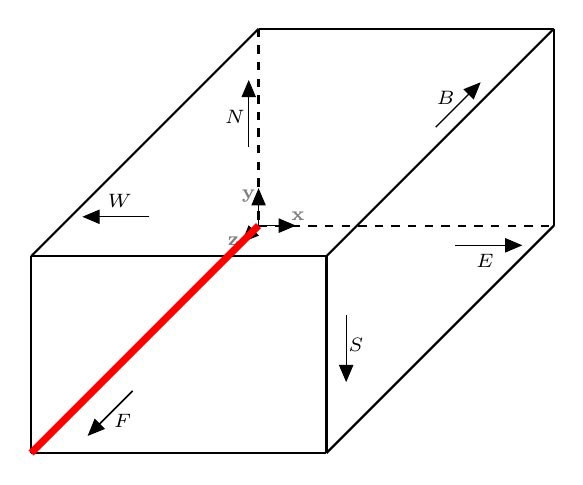
\begin{tikzpicture}[]
      \path pic[font=\scriptsize,scale=2.50]{geo};
      \draw[red,very thick,line width=0.9mm] (0,0,0) -- (0,0,7.5);
      % \draw[red,thick] (3.6,2.5,7.2) circle (0.5);
    \end{tikzpicture}
  }
  \subfloat[]{
    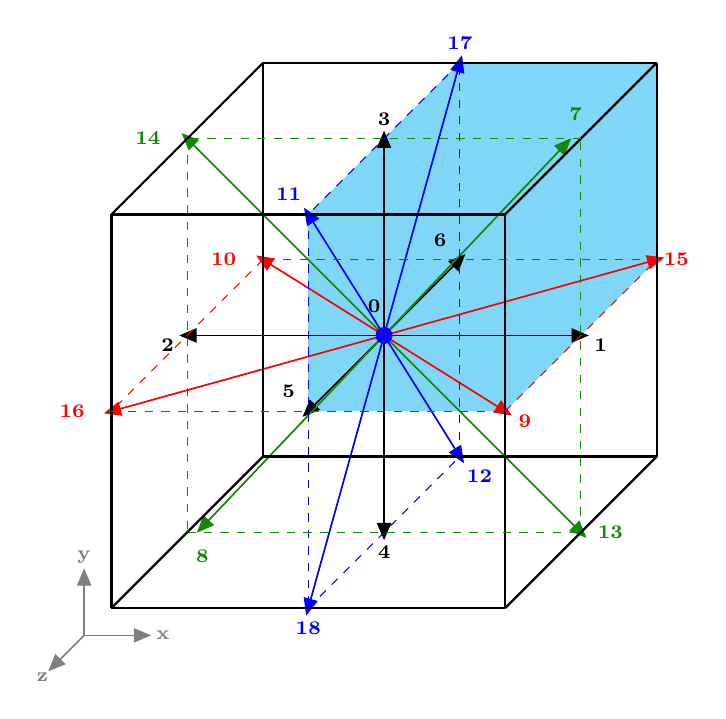
\begin{tikzpicture}[font=\scriptsize,scale=2.50,rotate around y=0,rotate around y=0]

      \fill[cyan!50] (1,1,1) -- (0,1,1) -- (0,0,1) -- (1,0,1) -- cycle; %  4.east-north-front
      \fill[cyan!50] (1,1,1) -- (0,1,1) -- (0,1,0) -- (1,1,0) -- cycle;
      \fill[cyan!50] (1,1,1) -- (1,1,0) -- (1,0,0) -- (1,0,1) -- cycle;
      \fill[cyan!50] (0,1,1) -- (0,1,0) -- (0,0,0) -- (0,0,1) -- cycle;
      \fill[cyan!50] (1,0,1) -- (0,0,1) -- (0,0,0) -- (1,0,0) -- cycle;
      \fill[cyan!50] (1,1,0) -- (0,1,0) -- (0,0, 0) -- (1,0,0) -- cycle;

      \fill[cyan!50] (1,1,-1) -- (0,1,-1) -- (0,0,-1) -- (1,0,-1) -- cycle; %  8. east-north-back
      \fill[cyan!50] (1,1,-1) -- (0,1,-1) -- (0,1,0) -- (1,1,0) -- cycle;
      \fill[cyan!50] (1,1,-1) -- (1,1,0) -- (1,0,0) -- (1,0,-1) -- cycle;
      \fill[cyan!50] (0,1,-1) -- (0,1,0) -- (0,0,0) -- (0,0,-1) -- cycle;
      \fill[cyan!50] (1,0,-1) -- (0,0,-1) -- (0,0,0) -- (1,0,0) -- cycle;
      \fill[cyan!50] (1,1,0) -- (0,1,0) -- (0,0, 0) -- (1,0,0) -- cycle;

      \path pic[font=\scriptsize,scale=2.50]{lat};
    \end{tikzpicture}
  }
  \caption{I=\{ 0,2,4,5,6,8,10,12,16,18\} and O=\{ 0,1,3,5,6,7,9,11,15,17\}}
\end{figure}

2. North-west
\begin{figure}[H]
  \centering

  \subfloat[]{
    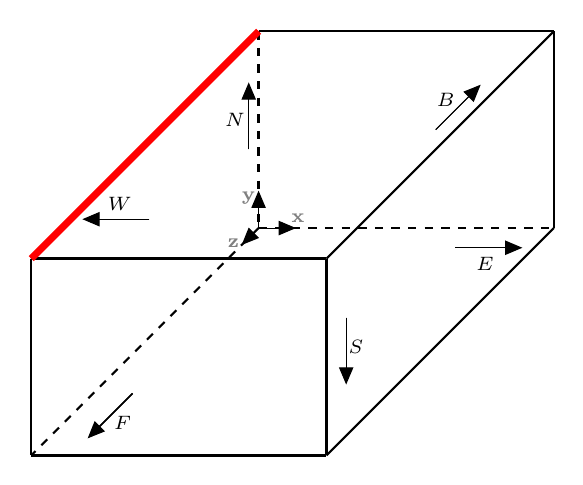
\begin{tikzpicture}[]
      \path pic[font=\scriptsize,scale=2.50]{geo};
      \draw[red,very thick,line width=0.9mm] (0,2.5,0) -- (0,2.5,7.5);
      % \draw[red,thick] (3.6,2.5,7.2) circle (0.5);
    \end{tikzpicture}
  }
  \subfloat[]{
    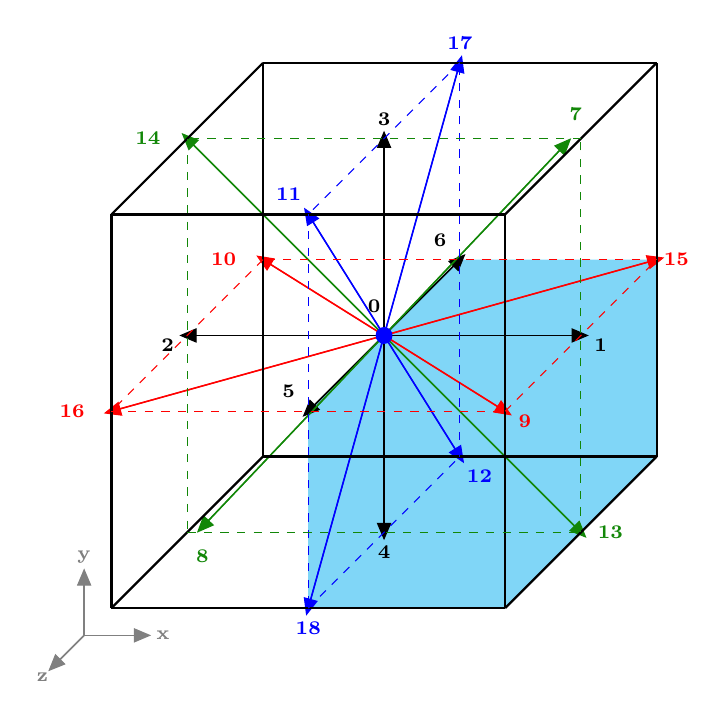
\begin{tikzpicture}[font=\scriptsize,scale=2.50,rotate around y=0,rotate around y=0]

      \fill[cyan!50] (0,-1,1) -- (1,-1,1) -- (1,0,1) -- (0,0,1) -- cycle;% 2. east-south-front
      \fill[cyan!50] (1,-1,1) -- (1,-1,0) -- (1,0,0) -- (1,0,1) -- cycle;
      \fill[cyan!50] (0,-1,1) -- (1,-1,1) -- (1,-1,0) -- (0,-1,0) -- cycle;
      \fill[cyan!50] (1,0,1) -- (0,0,1) -- (0,0,0) -- (1,0,0) -- cycle;
      \fill[cyan!50] (0,-1,0) -- (1,-1,0) -- (1,0, 0) -- (0,0,0) -- cycle;
      \fill[cyan!50] (0,-1,1) -- (0,-1,0) -- (0,0,0) -- (0,0,1) -- cycle;

      \fill[cyan!50] (1,-1,-1) -- (0,-1,-1) -- (0,0,-1) -- (1,0,-1) -- cycle; %  6.east-south-back
      \fill[cyan!50] (1,-1,-1) -- (0,-1,-1) -- (0,-1,0) -- (1,-1,0) -- cycle;
      \fill[cyan!50] (1,-1,-1) -- (1,-1,0) -- (1,0,0) -- (1,0,-1) -- cycle;
      \fill[cyan!50] (0,-1,-1) -- (0,-1,0) -- (0,0,0) -- (0,0,-1) -- cycle;
      \fill[cyan!50] (1,0,-1) -- (0,0,-1) -- (0,0,0) -- (1,0,0) -- cycle;
      \fill[cyan!50] (1,-1,0) -- (0,-1,0) -- (0,0, 0) -- (1,0,0) -- cycle;

      \path pic[font=\scriptsize,scale=2.50]{lat};
    \end{tikzpicture}
  }
  \caption{I=\{ 0,2,3,5,6,10,11,14,16,17\} and O=\{ 0,1,4,5,6,9,12,13,15,18\}}
\end{figure}

3. South-east
\begin{figure}[H]
  \centering

  \subfloat[]{
    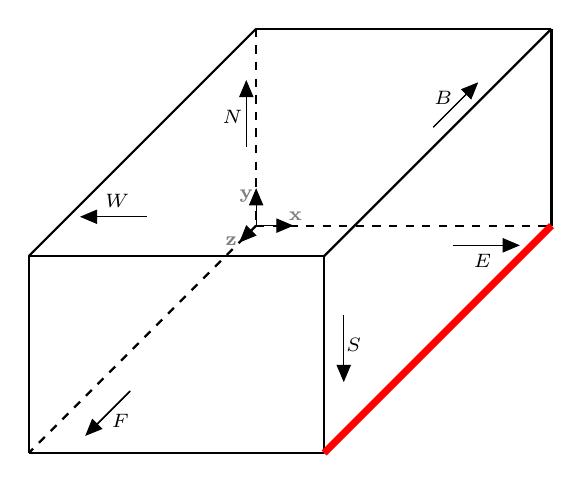
\begin{tikzpicture}[]
      \path pic[font=\scriptsize,scale=2.50]{geo};
      \draw[red,very thick,line width=0.9mm] (3.75,0,0) -- (3.75,0,7.5);
      % \draw[red,thick] (3.6,2.5,7.2) circle (0.5);
    \end{tikzpicture}
  }
  \subfloat[]{
    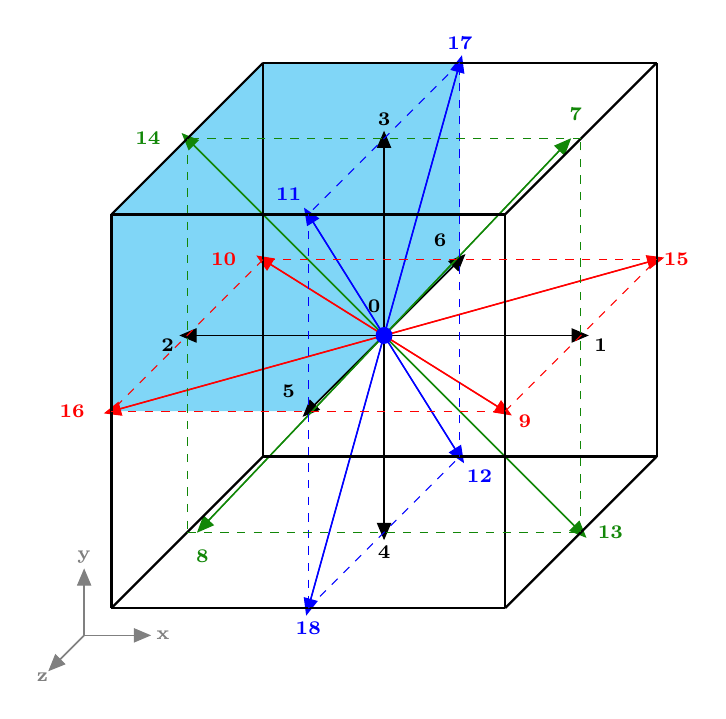
\begin{tikzpicture}[font=\scriptsize,scale=2.50,rotate around y=0,rotate around y=0]

      \fill[cyan!50] (-1,1,1) -- (0,1,1) -- (0,0,1) -- (-1,0,1) -- cycle; %  3.west-north-front
      \fill[cyan!50] (-1,1,1) -- (0,1,1) -- (0,1,0) -- (-1,1,0) -- cycle;
      \fill[cyan!50] (-1,1,1) -- (-1,1,0) -- (-1,0,0) -- (-1,0,1) -- cycle;
      \fill[cyan!50] (0,1,1) -- (0,1,0) -- (0,0,0) -- (0,0,1) -- cycle;
      \fill[cyan!50] (-1,0,1) -- (0,0,1) -- (0,0,0) -- (-1,0,0) -- cycle;
      \fill[cyan!50] (-1,1,0) -- (0,1,0) -- (0,0, 0) -- (-1,0,0) -- cycle;

      \fill[cyan!50] (-1,1,-1) -- (0,1,-1) -- (0,0,-1) -- (-1,0,-1) -- cycle; %  7.west-north-back
      \fill[cyan!50] (-1,1,-1) -- (0,1,-1) -- (0,1,0) -- (-1,1,0) -- cycle;
      \fill[cyan!50] (-1,1,-1) -- (-1,1,0) -- (-1,0,0) -- (-1,0,-1) -- cycle;
      \fill[cyan!50] (0,1,-1) -- (0,1,0) -- (0,0,0) -- (0,0,-1) -- cycle;
      \fill[cyan!50] (-1,0,-1) -- (0,0,-1) -- (0,0,0) -- (-1,0,0) -- cycle;
      \fill[cyan!50] (-1,1,0) -- (0,1,0) -- (0,0, 0) -- (-1,0,0) -- cycle;

      \path pic[font=\scriptsize,scale=2.50]{lat};
    \end{tikzpicture}
  }
  \caption{I=\{ 0,1,4,5,6,9,12,13,15,18\} and O=\{ 0,2,3,5,6,10,11,14,16,17\}}
\end{figure}

4. North-east
\begin{figure}[H]
  \centering

  \subfloat[]{
    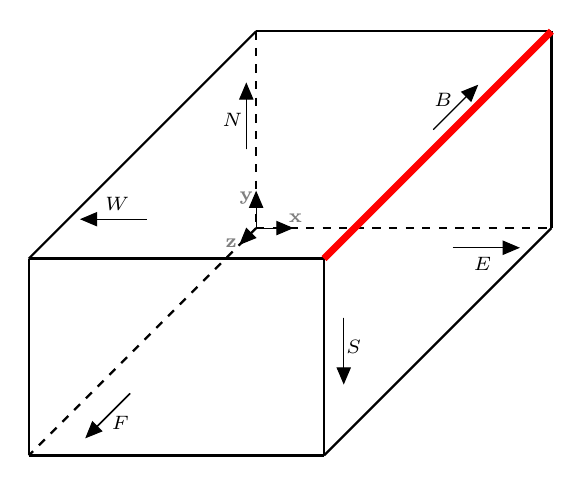
\begin{tikzpicture}[]
      \path pic[font=\scriptsize,scale=2.50]{geo};
      \draw[red,very thick,line width=0.9mm] (3.75,2.5,0) -- (3.75,2.5,7.5);
      % \draw[red,thick] (3.6,2.5,7.2) circle (0.5);
    \end{tikzpicture}
  }
  \subfloat[]{
    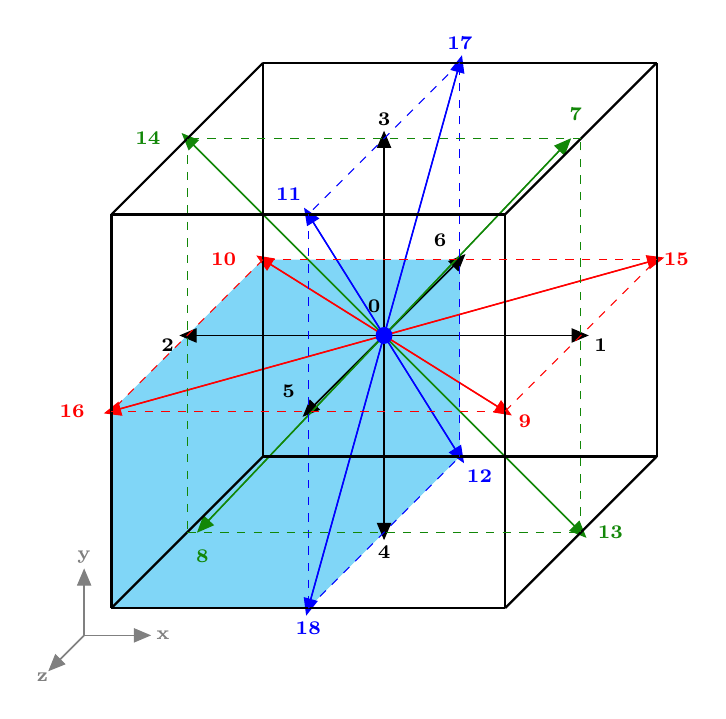
\begin{tikzpicture}[font=\scriptsize,scale=2.50,rotate around y=0,rotate around y=0]

      \fill[cyan!50] (-1,-1,1) -- (0,-1,1) -- (0,0,1) -- (-1,0,1) -- cycle; %  1.west-south-front
      \fill[cyan!50] (-1,-1,1) -- (0,-1,1) -- (0,-1,0) -- (-1,-1,0) -- cycle;
      \fill[cyan!50] (-1,-1,1) -- (-1,-1,0) -- (-1,0,0) -- (-1,0,1) -- cycle;
      \fill[cyan!50] (0,-1,1) -- (0,-1,0) -- (0,0,0) -- (0,0,1) -- cycle;
      \fill[cyan!50] (-1,0,1) -- (0,0,1) -- (0,0,0) -- (-1,0,0) -- cycle;
      \fill[cyan!50] (-1,-1,0) -- (0,-1,0) -- (0,0, 0) -- (-1,0,0) -- cycle;

      \fill[cyan!50] (-1,-1,-1) -- (0,-1,-1) -- (0,0,-1) -- (-1,0,-1) -- cycle; %  5. west-south-back
      \fill[cyan!50] (-1,-1,-1) -- (0,-1,-1) -- (0,-1,0) -- (-1,-1,0) -- cycle;
      \fill[cyan!50] (-1,-1,-1) -- (-1,-1,0) -- (-1,0,0) -- (-1,0,-1) -- cycle;
      \fill[cyan!50] (0,-1,-1) -- (0,-1,0) -- (0,0,0) -- (0,0,-1) -- cycle;
      \fill[cyan!50] (-1,0,-1) -- (0,0,-1) -- (0,0,0) -- (-1,0,0) -- cycle;
      \fill[cyan!50] (-1,-1,0) -- (0,-1,0) -- (0,0, 0) -- (-1,0,0) -- cycle;

      \path pic[font=\scriptsize,scale=2.50]{lat};
    \end{tikzpicture}
  }
  \caption{I=\{ 0,1,3,5,6,7,9,11,15,17\} and O=\{ 0,2,4,5,6,8,10,12,16,18\}}
\end{figure}

5. West-back
\begin{figure}[H]
  \centering

  \subfloat[]{
    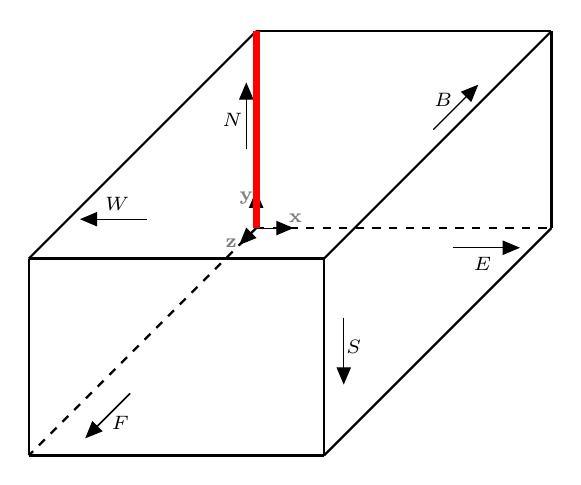
\begin{tikzpicture}[]
      \path pic[font=\scriptsize,scale=2.50]{geo};
      \draw[red,very thick,line width=0.9mm] (0,0,0) -- (0,2.5,0);
      % \draw[red,thick] (3.6,2.5,7.2) circle (0.5);
    \end{tikzpicture}
  }
  \subfloat[]{
    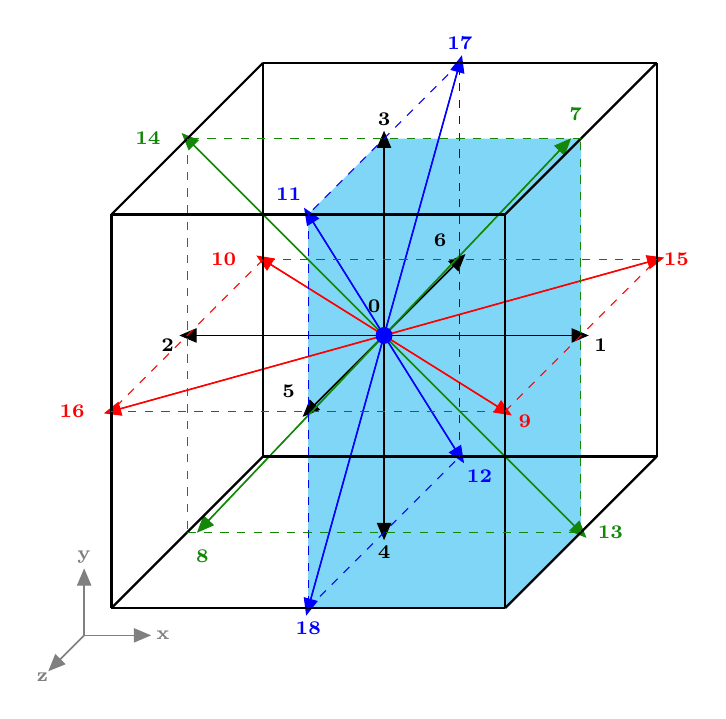
\begin{tikzpicture}[font=\scriptsize,scale=2.50,rotate around y=0,rotate around y=0]

      \fill[cyan!50] (0,-1,1) -- (1,-1,1) -- (1,0,1) -- (0,0,1) -- cycle;% 2. east-south-front
      \fill[cyan!50] (1,-1,1) -- (1,-1,0) -- (1,0,0) -- (1,0,1) -- cycle;
      \fill[cyan!50] (0,-1,1) -- (1,-1,1) -- (1,-1,0) -- (0,-1,0) -- cycle;
      \fill[cyan!50] (1,0,1) -- (0,0,1) -- (0,0,0) -- (1,0,0) -- cycle;
      \fill[cyan!50] (0,-1,0) -- (1,-1,0) -- (1,0, 0) -- (0,0,0) -- cycle;
      \fill[cyan!50] (0,-1,1) -- (0,-1,0) -- (0,0,0) -- (0,0,1) -- cycle;

      \fill[cyan!50] (1,1,1) -- (0,1,1) -- (0,0,1) -- (1,0,1) -- cycle; %  4.east-north-front
      \fill[cyan!50] (1,1,1) -- (0,1,1) -- (0,1,0) -- (1,1,0) -- cycle;
      \fill[cyan!50] (1,1,1) -- (1,1,0) -- (1,0,0) -- (1,0,1) -- cycle;
      \fill[cyan!50] (0,1,1) -- (0,1,0) -- (0,0,0) -- (0,0,1) -- cycle;
      \fill[cyan!50] (1,0,1) -- (0,0,1) -- (0,0,0) -- (1,0,0) -- cycle;
      \fill[cyan!50] (1,1,0) -- (0,1,0) -- (0,0, 0) -- (1,0,0) -- cycle;

      \path pic[font=\scriptsize,scale=2.50]{lat};
    \end{tikzpicture}
  }
  \caption{I=\{ 0,2,3,4,6,8,10,12,14,17\} and O=\{ 0,1,3,4,5,7,9,11,13,18\}}
\end{figure}

6. West-front
\begin{figure}[H]
  \centering

  \subfloat[]{
    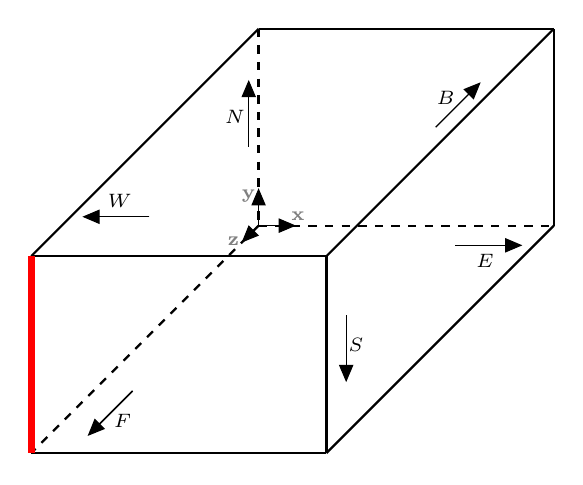
\begin{tikzpicture}[]
      \path pic[font=\scriptsize,scale=2.50]{geo};
      \draw[red,very thick,line width=0.9mm] (0,0,7.5) -- (0,2.5,7.5);
      % \draw[red,thick] (3.6,2.5,7.2) circle (0.5);
    \end{tikzpicture}
  }
  \subfloat[]{
    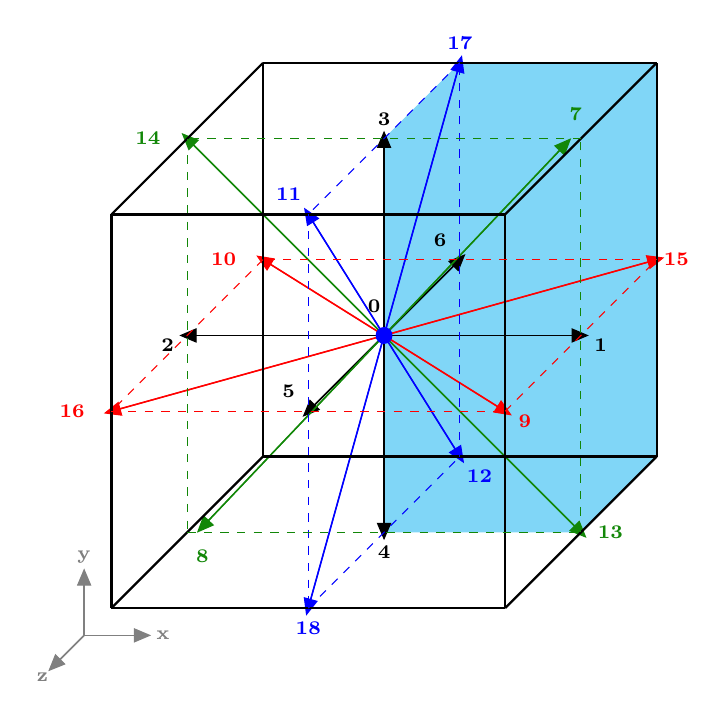
\begin{tikzpicture}[font=\scriptsize,scale=2.50,rotate around y=0,rotate around y=0]

      \fill[cyan!50] (1,-1,-1) -- (0,-1,-1) -- (0,0,-1) -- (1,0,-1) -- cycle; %  6.east-south-back
      \fill[cyan!50] (1,-1,-1) -- (0,-1,-1) -- (0,-1,0) -- (1,-1,0) -- cycle;
      \fill[cyan!50] (1,-1,-1) -- (1,-1,0) -- (1,0,0) -- (1,0,-1) -- cycle;
      \fill[cyan!50] (0,-1,-1) -- (0,-1,0) -- (0,0,0) -- (0,0,-1) -- cycle;
      \fill[cyan!50] (1,0,-1) -- (0,0,-1) -- (0,0,0) -- (1,0,0) -- cycle;
      \fill[cyan!50] (1,-1,0) -- (0,-1,0) -- (0,0, 0) -- (1,0,0) -- cycle;

      \fill[cyan!50] (1,1,-1) -- (0,1,-1) -- (0,0,-1) -- (1,0,-1) -- cycle; %  8. east-north-back
      \fill[cyan!50] (1,1,-1) -- (0,1,-1) -- (0,1,0) -- (1,1,0) -- cycle;
      \fill[cyan!50] (1,1,-1) -- (1,1,0) -- (1,0,0) -- (1,0,-1) -- cycle;
      \fill[cyan!50] (0,1,-1) -- (0,1,0) -- (0,0,0) -- (0,0,-1) -- cycle;
      \fill[cyan!50] (1,0,-1) -- (0,0,-1) -- (0,0,0) -- (1,0,0) -- cycle;
      \fill[cyan!50] (1,1,0) -- (0,1,0) -- (0,0, 0) -- (1,0,0) -- cycle;

      \path pic[font=\scriptsize,scale=2.50]{lat};
    \end{tikzpicture}
  }
  \caption{I=\{ 0,2,3,4,5,8,11,14,16,18\} and O=\{ 0,1,3,4,6,7,12,13,15,17\}}
\end{figure}

7. East-back
\begin{figure}[H]
  \centering

  \subfloat[]{
    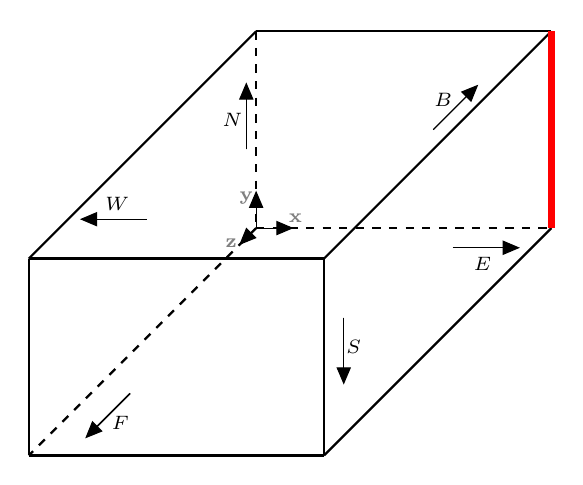
\begin{tikzpicture}[]
      \path pic[font=\scriptsize,scale=2.50]{geo};
      \draw[red,very thick,line width=0.9mm] (3.75,0,0) -- (3.75,2.5,0);
      % \draw[red,thick] (3.6,2.5,7.2) circle (0.5);
    \end{tikzpicture}
  }
  \subfloat[]{
    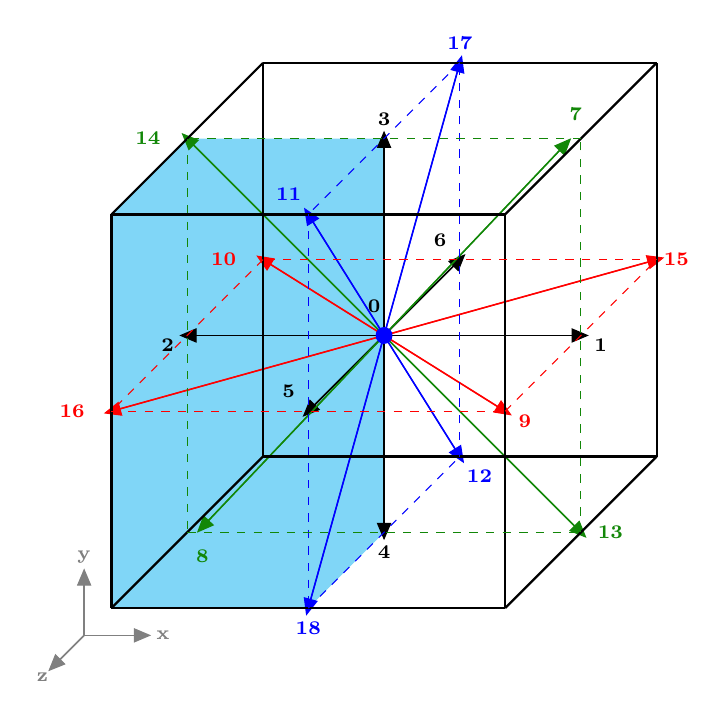
\begin{tikzpicture}[font=\scriptsize,scale=2.50,rotate around y=0,rotate around y=0]

      \fill[cyan!50] (-1,-1,1) -- (0,-1,1) -- (0,0,1) -- (-1,0,1) -- cycle; %  1.west-south-front
      \fill[cyan!50] (-1,-1,1) -- (0,-1,1) -- (0,-1,0) -- (-1,-1,0) -- cycle;
      \fill[cyan!50] (-1,-1,1) -- (-1,-1,0) -- (-1,0,0) -- (-1,0,1) -- cycle;
      \fill[cyan!50] (0,-1,1) -- (0,-1,0) -- (0,0,0) -- (0,0,1) -- cycle;
      \fill[cyan!50] (-1,0,1) -- (0,0,1) -- (0,0,0) -- (-1,0,0) -- cycle;
      \fill[cyan!50] (-1,-1,0) -- (0,-1,0) -- (0,0, 0) -- (-1,0,0) -- cycle;

      \fill[cyan!50] (-1,1,1) -- (0,1,1) -- (0,0,1) -- (-1,0,1) -- cycle; %  3.west-north-front
      \fill[cyan!50] (-1,1,1) -- (0,1,1) -- (0,1,0) -- (-1,1,0) -- cycle;
      \fill[cyan!50] (-1,1,1) -- (-1,1,0) -- (-1,0,0) -- (-1,0,1) -- cycle;
      \fill[cyan!50] (0,1,1) -- (0,1,0) -- (0,0,0) -- (0,0,1) -- cycle;
      \fill[cyan!50] (-1,0,1) -- (0,0,1) -- (0,0,0) -- (-1,0,0) -- cycle;
      \fill[cyan!50] (-1,1,0) -- (0,1,0) -- (0,0, 0) -- (-1,0,0) -- cycle;

      \path pic[font=\scriptsize,scale=2.50]{lat};
    \end{tikzpicture}
  }
  \caption{I=\{ 0,1,3,4,6,7,12,13,15,17\} and O=\{ 0,2,3,4,5,8,11,14,16,18\}}
\end{figure}

8. East-front
\begin{figure}[H]
  \centering

  \subfloat[]{
    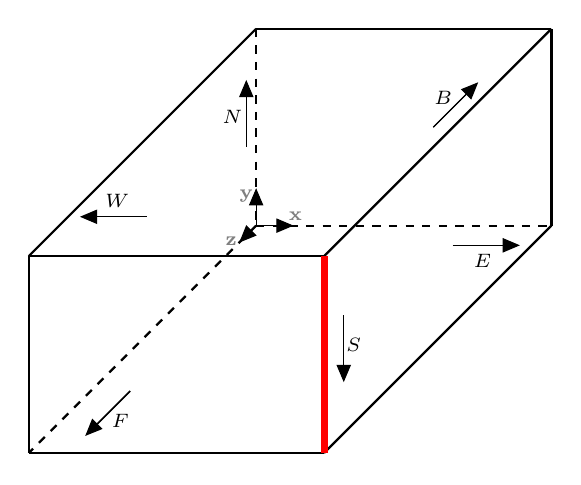
\begin{tikzpicture}[]
      \path pic[font=\scriptsize,scale=2.50]{geo};
      \draw[red,very thick,line width=0.9mm] (3.75,0,7.5) -- (3.75,2.5,7.5);
      % \draw[red,thick] (3.6,2.5,7.2) circle (0.5);
    \end{tikzpicture}
  }
  \subfloat[]{
    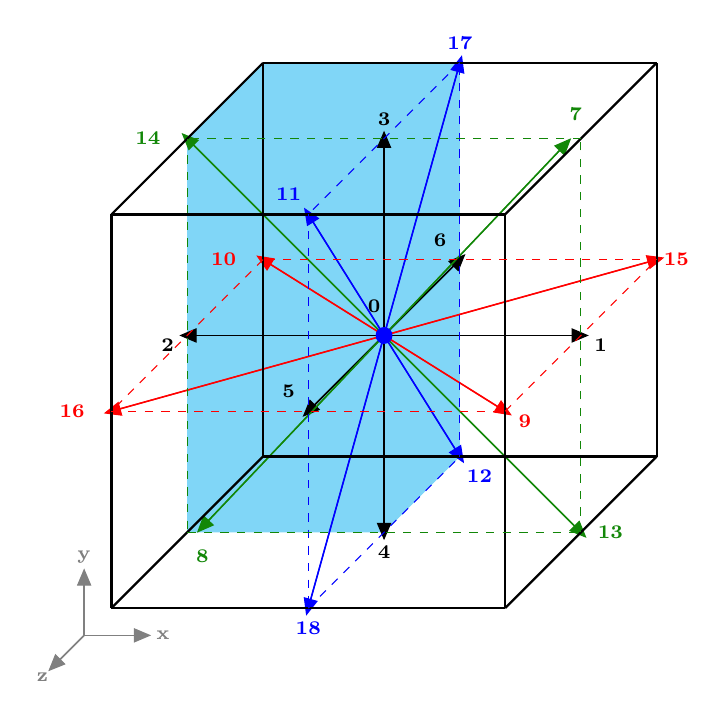
\begin{tikzpicture}[font=\scriptsize,scale=2.50,rotate around y=0,rotate around y=0]

      \fill[cyan!50] (-1,-1,-1) -- (0,-1,-1) -- (0,0,-1) -- (-1,0,-1) -- cycle; %  5. west-south-back
      \fill[cyan!50] (-1,-1,-1) -- (0,-1,-1) -- (0,-1,0) -- (-1,-1,0) -- cycle;
      \fill[cyan!50] (-1,-1,-1) -- (-1,-1,0) -- (-1,0,0) -- (-1,0,-1) -- cycle;
      \fill[cyan!50] (0,-1,-1) -- (0,-1,0) -- (0,0,0) -- (0,0,-1) -- cycle;
      \fill[cyan!50] (-1,0,-1) -- (0,0,-1) -- (0,0,0) -- (-1,0,0) -- cycle;
      \fill[cyan!50] (-1,-1,0) -- (0,-1,0) -- (0,0, 0) -- (-1,0,0) -- cycle;

      \fill[cyan!50] (-1,1,-1) -- (0,1,-1) -- (0,0,-1) -- (-1,0,-1) -- cycle; %  7.west-north-back
      \fill[cyan!50] (-1,1,-1) -- (0,1,-1) -- (0,1,0) -- (-1,1,0) -- cycle;
      \fill[cyan!50] (-1,1,-1) -- (-1,1,0) -- (-1,0,0) -- (-1,0,-1) -- cycle;
      \fill[cyan!50] (0,1,-1) -- (0,1,0) -- (0,0,0) -- (0,0,-1) -- cycle;
      \fill[cyan!50] (-1,0,-1) -- (0,0,-1) -- (0,0,0) -- (-1,0,0) -- cycle;
      \fill[cyan!50] (-1,1,0) -- (0,1,0) -- (0,0, 0) -- (-1,0,0) -- cycle;

      \path pic[font=\scriptsize,scale=2.50]{lat};
    \end{tikzpicture}
  }
  \caption{I=\{ 0,1,3,4,5,7,9,11,13,18\} and O=\{ 0,2,3,4,6,8,10,12,14,17\}}
\end{figure}

9. south-back
\begin{figure}[H]
  \centering

  \subfloat[]{
    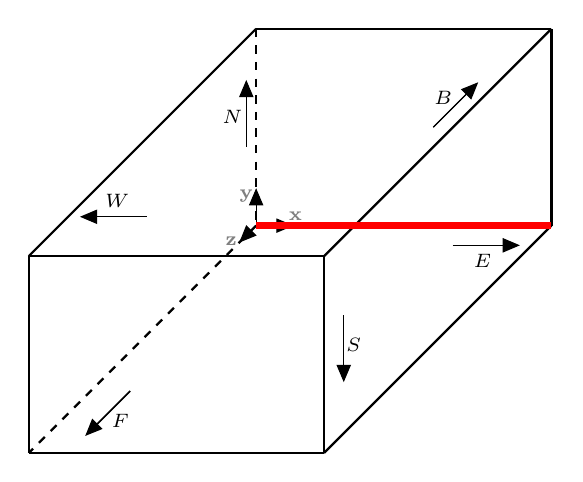
\begin{tikzpicture}[]
      \path pic[font=\scriptsize,scale=2.50]{geo};
      \draw[red,very thick,line width=0.9mm] (0,0,0) -- (3.75,0,0);
      % \draw[red,thick] (3.6,2.5,7.2) circle (0.5);
    \end{tikzpicture}
  }
  \subfloat[]{
    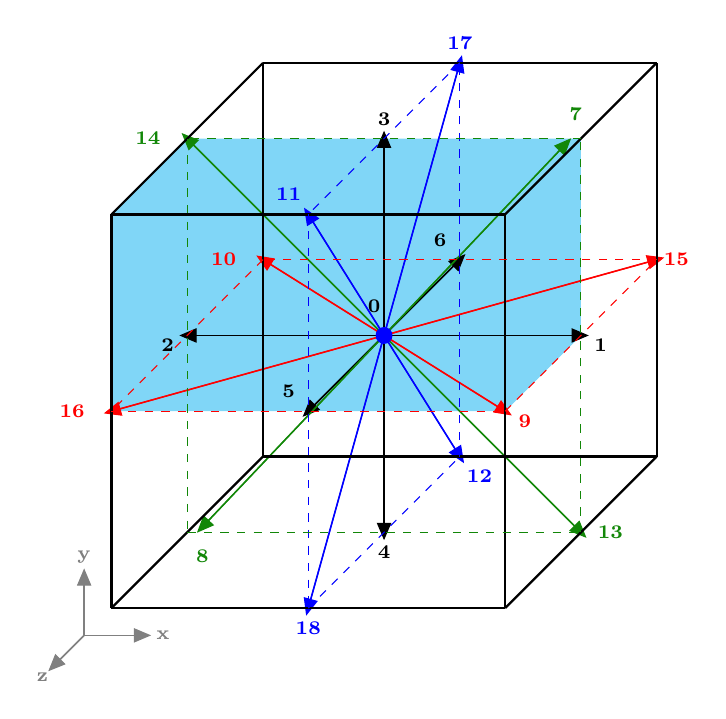
\begin{tikzpicture}[font=\scriptsize,scale=2.50,rotate around y=0,rotate around y=0]

      \fill[cyan!50] (-1,1,1) -- (0,1,1) -- (0,0,1) -- (-1,0,1) -- cycle; %  3.west-north-front
      \fill[cyan!50] (-1,1,1) -- (0,1,1) -- (0,1,0) -- (-1,1,0) -- cycle;
      \fill[cyan!50] (-1,1,1) -- (-1,1,0) -- (-1,0,0) -- (-1,0,1) -- cycle;
      \fill[cyan!50] (0,1,1) -- (0,1,0) -- (0,0,0) -- (0,0,1) -- cycle;
      \fill[cyan!50] (-1,0,1) -- (0,0,1) -- (0,0,0) -- (-1,0,0) -- cycle;
      \fill[cyan!50] (-1,1,0) -- (0,1,0) -- (0,0, 0) -- (-1,0,0) -- cycle;

      \fill[cyan!50] (1,1,1) -- (0,1,1) -- (0,0,1) -- (1,0,1) -- cycle; %  4.east-north-front
      \fill[cyan!50] (1,1,1) -- (0,1,1) -- (0,1,0) -- (1,1,0) -- cycle;
      \fill[cyan!50] (1,1,1) -- (1,1,0) -- (1,0,0) -- (1,0,1) -- cycle;
      \fill[cyan!50] (0,1,1) -- (0,1,0) -- (0,0,0) -- (0,0,1) -- cycle;
      \fill[cyan!50] (1,0,1) -- (0,0,1) -- (0,0,0) -- (1,0,0) -- cycle;
      \fill[cyan!50] (1,1,0) -- (0,1,0) -- (0,0, 0) -- (1,0,0) -- cycle;

      \path pic[font=\scriptsize,scale=2.50]{lat};
    \end{tikzpicture}
  }
  \caption{I=\{ 0,1,2,4,6,8,10,12,13,15\} and O=\{ 0,1,2,3,5,7,9,11,14,16\}}
\end{figure}

10. south-front
\begin{figure}[H]
  \centering

  \subfloat[]{
    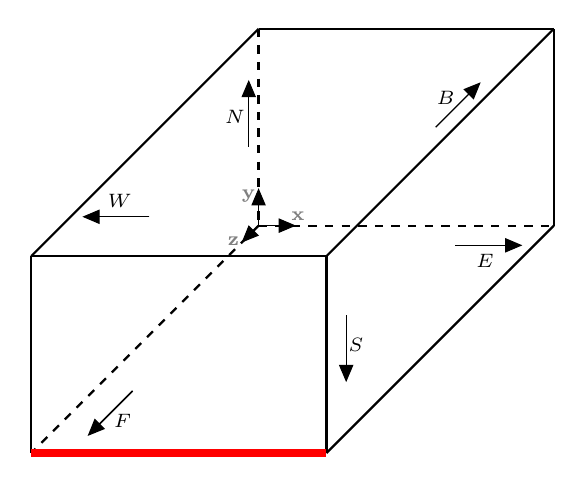
\begin{tikzpicture}[]
      \path pic[font=\scriptsize,scale=2.50]{geo};
      \draw[red,very thick,line width=0.9mm] (0,0,7.5) -- (3.75,0,7.5);
      % \draw[red,thick] (3.6,2.5,7.2) circle (0.5);
    \end{tikzpicture}
  }
  \subfloat[]{
    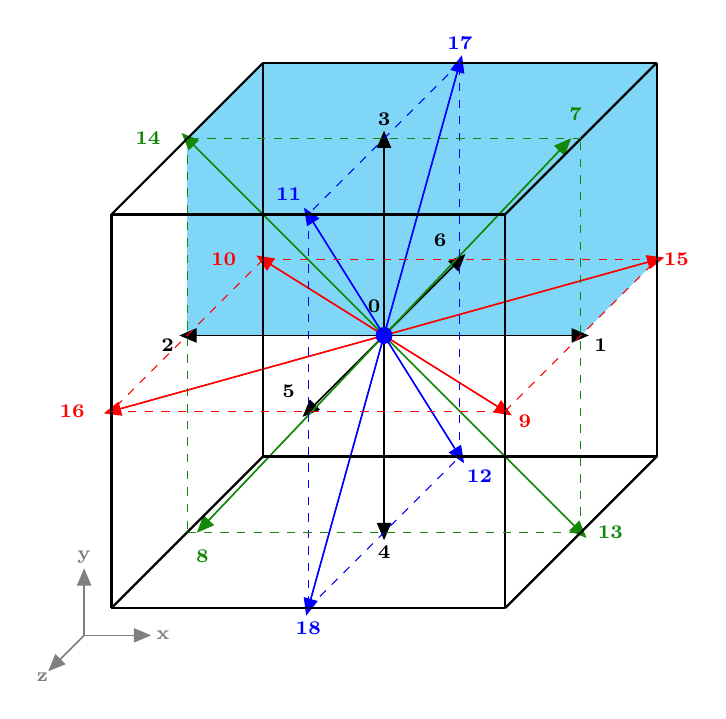
\begin{tikzpicture}[font=\scriptsize,scale=2.50,rotate around y=0,rotate around y=0]

      \fill[cyan!50] (-1,1,-1) -- (0,1,-1) -- (0,0,-1) -- (-1,0,-1) -- cycle; %  7.west-north-back
      \fill[cyan!50] (-1,1,-1) -- (0,1,-1) -- (0,1,0) -- (-1,1,0) -- cycle;
      \fill[cyan!50] (-1,1,-1) -- (-1,1,0) -- (-1,0,0) -- (-1,0,-1) -- cycle;
      \fill[cyan!50] (0,1,-1) -- (0,1,0) -- (0,0,0) -- (0,0,-1) -- cycle;
      \fill[cyan!50] (-1,0,-1) -- (0,0,-1) -- (0,0,0) -- (-1,0,0) -- cycle;
      \fill[cyan!50] (-1,1,0) -- (0,1,0) -- (0,0, 0) -- (-1,0,0) -- cycle;

      \fill[cyan!50] (1,1,-1) -- (0,1,-1) -- (0,0,-1) -- (1,0,-1) -- cycle; %  8. east-north-back
      \fill[cyan!50] (1,1,-1) -- (0,1,-1) -- (0,1,0) -- (1,1,0) -- cycle;
      \fill[cyan!50] (1,1,-1) -- (1,1,0) -- (1,0,0) -- (1,0,-1) -- cycle;
      \fill[cyan!50] (0,1,-1) -- (0,1,0) -- (0,0,0) -- (0,0,-1) -- cycle;
      \fill[cyan!50] (1,0,-1) -- (0,0,-1) -- (0,0,0) -- (1,0,0) -- cycle;
      \fill[cyan!50] (1,1,0) -- (0,1,0) -- (0,0, 0) -- (1,0,0) -- cycle;

      \path pic[font=\scriptsize,scale=2.50]{lat};
    \end{tikzpicture}
  }
  \caption{I=\{ 0,1,2,4,5,8,9,13,16,18\} and O=\{ 0,1,2,3,6,7,10,14,15,17\}}
\end{figure}

11. north-back
\begin{figure}[H]
  \centering

  \subfloat[]{
    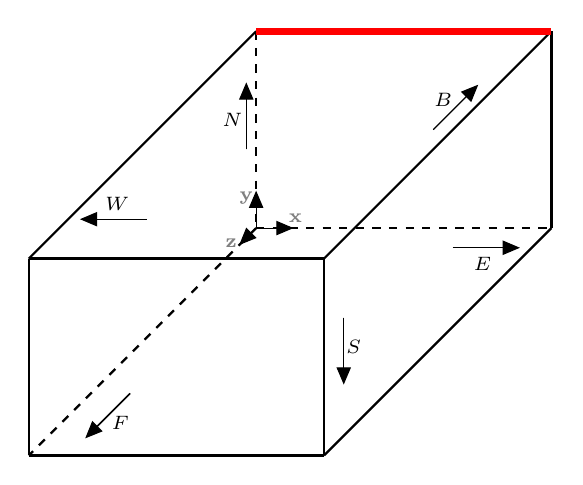
\begin{tikzpicture}[]
      \path pic[font=\scriptsize,scale=2.50]{geo};
      \draw[red,very thick,line width=0.9mm] (0,2.5,0) -- (3.75,2.5,0);
      % \draw[red,thick] (3.6,2.5,7.2) circle (0.5);
    \end{tikzpicture}
  }
  \subfloat[]{
    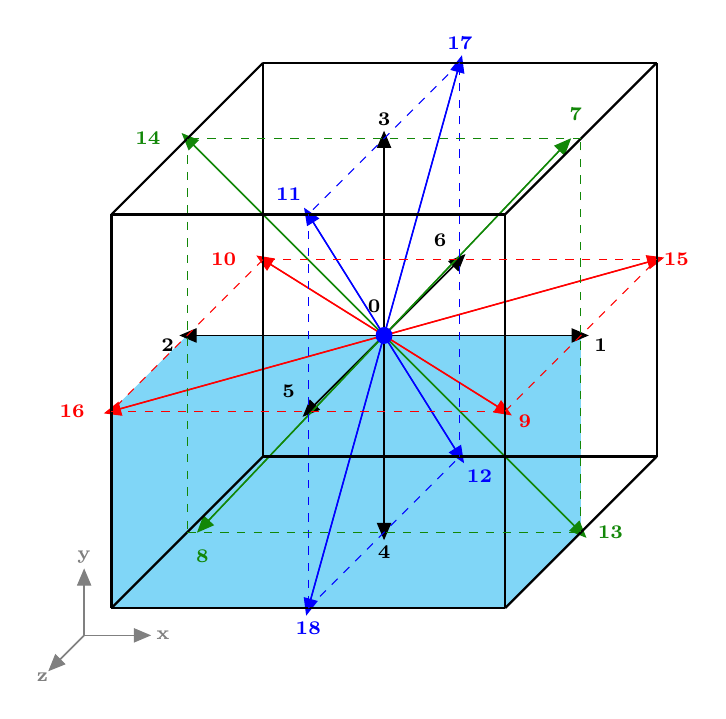
\begin{tikzpicture}[font=\scriptsize,scale=2.50,rotate around y=0,rotate around y=0]

      \fill[cyan!50] (-1,-1,1) -- (0,-1,1) -- (0,0,1) -- (-1,0,1) -- cycle; %  1.west-south-front
      \fill[cyan!50] (-1,-1,1) -- (0,-1,1) -- (0,-1,0) -- (-1,-1,0) -- cycle;
      \fill[cyan!50] (-1,-1,1) -- (-1,-1,0) -- (-1,0,0) -- (-1,0,1) -- cycle;
      \fill[cyan!50] (0,-1,1) -- (0,-1,0) -- (0,0,0) -- (0,0,1) -- cycle;
      \fill[cyan!50] (-1,0,1) -- (0,0,1) -- (0,0,0) -- (-1,0,0) -- cycle;
      \fill[cyan!50] (-1,-1,0) -- (0,-1,0) -- (0,0, 0) -- (-1,0,0) -- cycle;

      \fill[cyan!50] (0,-1,1) -- (1,-1,1) -- (1,0,1) -- (0,0,1) -- cycle;% 2. east-south-front
      \fill[cyan!50] (1,-1,1) -- (1,-1,0) -- (1,0,0) -- (1,0,1) -- cycle;
      \fill[cyan!50] (0,-1,1) -- (1,-1,1) -- (1,-1,0) -- (0,-1,0) -- cycle;
      \fill[cyan!50] (1,0,1) -- (0,0,1) -- (0,0,0) -- (1,0,0) -- cycle;
      \fill[cyan!50] (0,-1,0) -- (1,-1,0) -- (1,0, 0) -- (0,0,0) -- cycle;
      \fill[cyan!50] (0,-1,1) -- (0,-1,0) -- (0,0,0) -- (0,0,1) -- cycle;

      \path pic[font=\scriptsize,scale=2.50]{lat};
    \end{tikzpicture}
  }
  \caption{I=\{ 0,1,2,3,6,7,10,14,15,17\} and O=\{ 0,1,2,4,5,8,9,13,16,18\}}
\end{figure}

12. north-front
\begin{figure}[H]
  \centering

  \subfloat[]{
    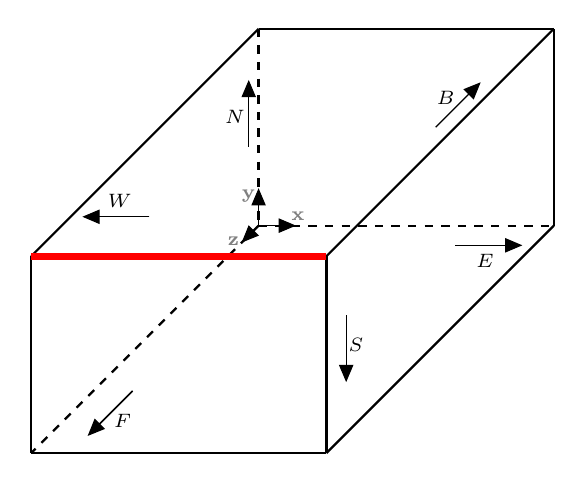
\begin{tikzpicture}[]
      \path pic[font=\scriptsize,scale=2.50]{geo};
      \draw[red,very thick,line width=0.9mm] (0,2.5,7.5) -- (3.75,2.5,7.5);
      % \draw[red,thick] (3.6,2.5,7.2) circle (0.5);
    \end{tikzpicture}
  }
  \subfloat[]{
    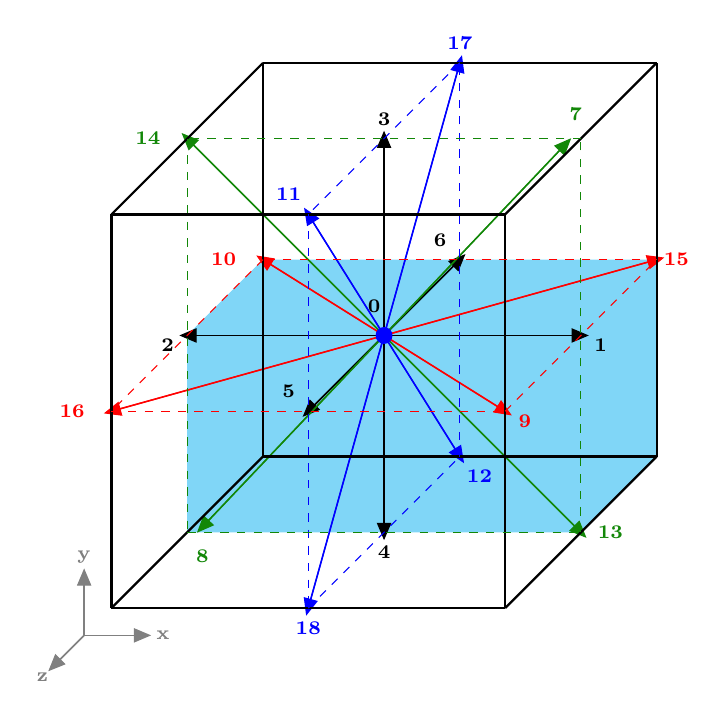
\begin{tikzpicture}[font=\scriptsize,scale=2.50,rotate around y=0,rotate around y=0]

      \fill[cyan!50] (-1,-1,-1) -- (0,-1,-1) -- (0,0,-1) -- (-1,0,-1) -- cycle; %  5. west-south-back
      \fill[cyan!50] (-1,-1,-1) -- (0,-1,-1) -- (0,-1,0) -- (-1,-1,0) -- cycle;
      \fill[cyan!50] (-1,-1,-1) -- (-1,-1,0) -- (-1,0,0) -- (-1,0,-1) -- cycle;
      \fill[cyan!50] (0,-1,-1) -- (0,-1,0) -- (0,0,0) -- (0,0,-1) -- cycle;
      \fill[cyan!50] (-1,0,-1) -- (0,0,-1) -- (0,0,0) -- (-1,0,0) -- cycle;
      \fill[cyan!50] (-1,-1,0) -- (0,-1,0) -- (0,0, 0) -- (-1,0,0) -- cycle;

      \fill[cyan!50] (1,-1,-1) -- (0,-1,-1) -- (0,0,-1) -- (1,0,-1) -- cycle; %  6.east-south-back
      \fill[cyan!50] (1,-1,-1) -- (0,-1,-1) -- (0,-1,0) -- (1,-1,0) -- cycle;
      \fill[cyan!50] (1,-1,-1) -- (1,-1,0) -- (1,0,0) -- (1,0,-1) -- cycle;
      \fill[cyan!50] (0,-1,-1) -- (0,-1,0) -- (0,0,0) -- (0,0,-1) -- cycle;
      \fill[cyan!50] (1,0,-1) -- (0,0,-1) -- (0,0,0) -- (1,0,0) -- cycle;
      \fill[cyan!50] (1,-1,0) -- (0,-1,0) -- (0,0, 0) -- (1,0,0) -- cycle;

      \path pic[font=\scriptsize,scale=2.50]{lat};
    \end{tikzpicture}
  }
  \caption{I=\{ 0,1,2,3,5,7,9,11,14,16\} and O=\{ 0,1,2,4,6,8,10,12,13,15\}}
\end{figure}

\cleardoublepage
%=======================================================================================

\begin{center}
  \Large{\textbf{Faces}}
\end{center}

1. West
\begin{figure}[H]
  \centering

  \subfloat[]{
    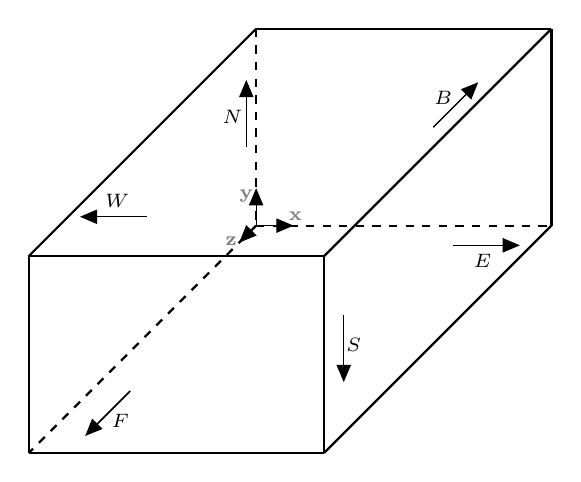
\begin{tikzpicture}[]
      \path pic[font=\scriptsize,scale=2.50]{geo};
    \end{tikzpicture}
  }
  \subfloat[]{
    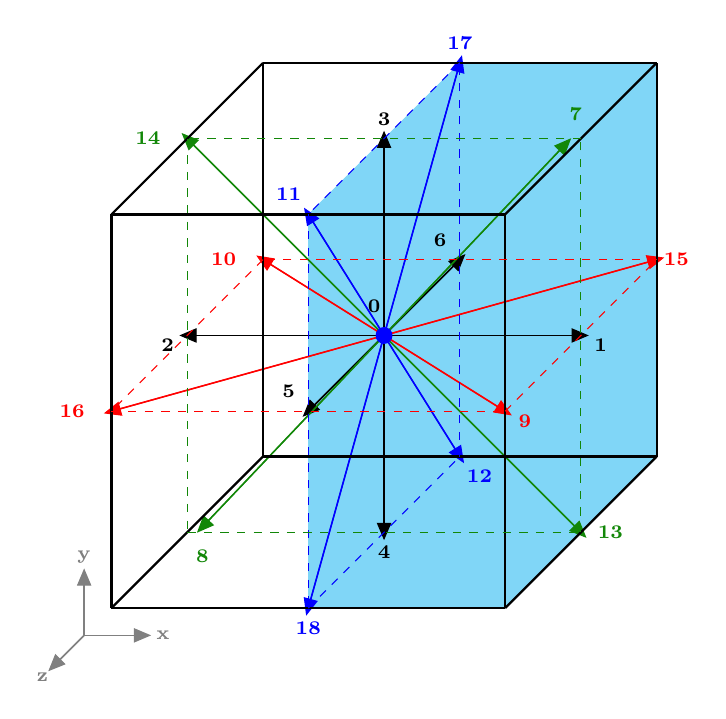
\begin{tikzpicture}[font=\scriptsize,scale=2.50,rotate around y=0,rotate around y=0]

      \fill[cyan!50] (0,-1,1) -- (1,-1,1) -- (1,0,1) -- (0,0,1) -- cycle;% 2. east-south-front
      \fill[cyan!50] (1,-1,1) -- (1,-1,0) -- (1,0,0) -- (1,0,1) -- cycle;
      \fill[cyan!50] (0,-1,1) -- (1,-1,1) -- (1,-1,0) -- (0,-1,0) -- cycle;
      \fill[cyan!50] (1,0,1) -- (0,0,1) -- (0,0,0) -- (1,0,0) -- cycle;
      \fill[cyan!50] (0,-1,0) -- (1,-1,0) -- (1,0, 0) -- (0,0,0) -- cycle;
      \fill[cyan!50] (0,-1,1) -- (0,-1,0) -- (0,0,0) -- (0,0,1) -- cycle;

      \fill[cyan!50] (1,1,1) -- (0,1,1) -- (0,0,1) -- (1,0,1) -- cycle; %  4.east-north-front
      \fill[cyan!50] (1,1,1) -- (0,1,1) -- (0,1,0) -- (1,1,0) -- cycle;
      \fill[cyan!50] (1,1,1) -- (1,1,0) -- (1,0,0) -- (1,0,1) -- cycle;
      \fill[cyan!50] (0,1,1) -- (0,1,0) -- (0,0,0) -- (0,0,1) -- cycle;
      \fill[cyan!50] (1,0,1) -- (0,0,1) -- (0,0,0) -- (1,0,0) -- cycle;
      \fill[cyan!50] (1,1,0) -- (0,1,0) -- (0,0, 0) -- (1,0,0) -- cycle;

      \fill[cyan!50] (1,-1,-1) -- (0,-1,-1) -- (0,0,-1) -- (1,0,-1) -- cycle; %  6.east-south-back
      \fill[cyan!50] (1,-1,-1) -- (0,-1,-1) -- (0,-1,0) -- (1,-1,0) -- cycle;
      \fill[cyan!50] (1,-1,-1) -- (1,-1,0) -- (1,0,0) -- (1,0,-1) -- cycle;
      \fill[cyan!50] (0,-1,-1) -- (0,-1,0) -- (0,0,0) -- (0,0,-1) -- cycle;
      \fill[cyan!50] (1,0,-1) -- (0,0,-1) -- (0,0,0) -- (1,0,0) -- cycle;
      \fill[cyan!50] (1,-1,0) -- (0,-1,0) -- (0,0, 0) -- (1,0,0) -- cycle;

      \fill[cyan!50] (1,1,-1) -- (0,1,-1) -- (0,0,-1) -- (1,0,-1) -- cycle; %  8. east-north-back
      \fill[cyan!50] (1,1,-1) -- (0,1,-1) -- (0,1,0) -- (1,1,0) -- cycle;
      \fill[cyan!50] (1,1,-1) -- (1,1,0) -- (1,0,0) -- (1,0,-1) -- cycle;
      \fill[cyan!50] (0,1,-1) -- (0,1,0) -- (0,0,0) -- (0,0,-1) -- cycle;
      \fill[cyan!50] (1,0,-1) -- (0,0,-1) -- (0,0,0) -- (1,0,0) -- cycle;
      \fill[cyan!50] (1,1,0) -- (0,1,0) -- (0,0, 0) -- (1,0,0) -- cycle;

      \path pic[font=\scriptsize,scale=2.50]{lat};
    \end{tikzpicture}
  }
  \caption{I=\{ 0,2,3,4,5,6,8,10,11,12,14,16,17,18\} and O=\{ 0,1,3,4,5,6,7,9,11,12,13,15,17,18\}}
\end{figure}

2. East
\begin{figure}[H]
  \centering

  \subfloat[]{
    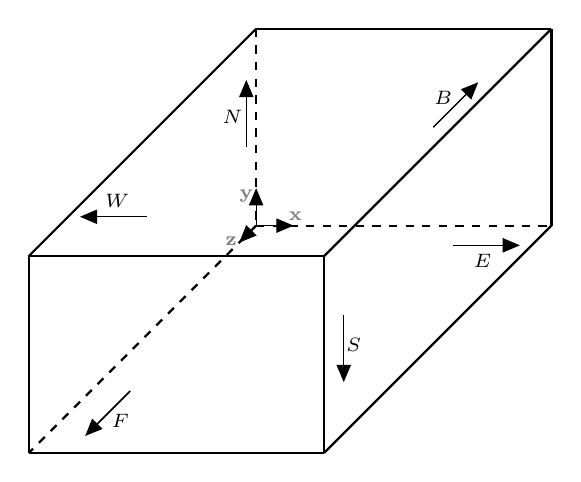
\begin{tikzpicture}[]
      \path pic[font=\scriptsize,scale=2.50]{geo};
    \end{tikzpicture}
  }
  \subfloat[]{
    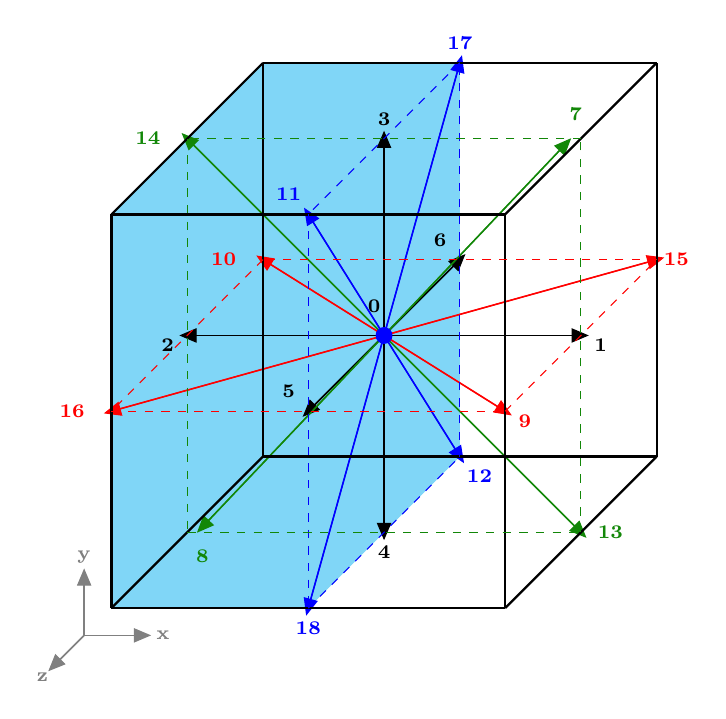
\begin{tikzpicture}[font=\scriptsize,scale=2.50,rotate around y=0,rotate around y=0]

      \fill[cyan!50] (-1,-1,1) -- (0,-1,1) -- (0,0,1) -- (-1,0,1) -- cycle; %  1.west-south-front
      \fill[cyan!50] (-1,-1,1) -- (0,-1,1) -- (0,-1,0) -- (-1,-1,0) -- cycle;
      \fill[cyan!50] (-1,-1,1) -- (-1,-1,0) -- (-1,0,0) -- (-1,0,1) -- cycle;
      \fill[cyan!50] (0,-1,1) -- (0,-1,0) -- (0,0,0) -- (0,0,1) -- cycle;
      \fill[cyan!50] (-1,0,1) -- (0,0,1) -- (0,0,0) -- (-1,0,0) -- cycle;
      \fill[cyan!50] (-1,-1,0) -- (0,-1,0) -- (0,0, 0) -- (-1,0,0) -- cycle;

      \fill[cyan!50] (-1,1,1) -- (0,1,1) -- (0,0,1) -- (-1,0,1) -- cycle; %  3.west-north-front
      \fill[cyan!50] (-1,1,1) -- (0,1,1) -- (0,1,0) -- (-1,1,0) -- cycle;
      \fill[cyan!50] (-1,1,1) -- (-1,1,0) -- (-1,0,0) -- (-1,0,1) -- cycle;
      \fill[cyan!50] (0,1,1) -- (0,1,0) -- (0,0,0) -- (0,0,1) -- cycle;
      \fill[cyan!50] (-1,0,1) -- (0,0,1) -- (0,0,0) -- (-1,0,0) -- cycle;
      \fill[cyan!50] (-1,1,0) -- (0,1,0) -- (0,0, 0) -- (-1,0,0) -- cycle;

      \fill[cyan!50] (-1,-1,-1) -- (0,-1,-1) -- (0,0,-1) -- (-1,0,-1) -- cycle; %  5. west-south-back
      \fill[cyan!50] (-1,-1,-1) -- (0,-1,-1) -- (0,-1,0) -- (-1,-1,0) -- cycle;
      \fill[cyan!50] (-1,-1,-1) -- (-1,-1,0) -- (-1,0,0) -- (-1,0,-1) -- cycle;
      \fill[cyan!50] (0,-1,-1) -- (0,-1,0) -- (0,0,0) -- (0,0,-1) -- cycle;
      \fill[cyan!50] (-1,0,-1) -- (0,0,-1) -- (0,0,0) -- (-1,0,0) -- cycle;
      \fill[cyan!50] (-1,-1,0) -- (0,-1,0) -- (0,0, 0) -- (-1,0,0) -- cycle;

      \fill[cyan!50] (-1,1,-1) -- (0,1,-1) -- (0,0,-1) -- (-1,0,-1) -- cycle; %  7.west-north-back
      \fill[cyan!50] (-1,1,-1) -- (0,1,-1) -- (0,1,0) -- (-1,1,0) -- cycle;
      \fill[cyan!50] (-1,1,-1) -- (-1,1,0) -- (-1,0,0) -- (-1,0,-1) -- cycle;
      \fill[cyan!50] (0,1,-1) -- (0,1,0) -- (0,0,0) -- (0,0,-1) -- cycle;
      \fill[cyan!50] (-1,0,-1) -- (0,0,-1) -- (0,0,0) -- (-1,0,0) -- cycle;
      \fill[cyan!50] (-1,1,0) -- (0,1,0) -- (0,0, 0) -- (-1,0,0) -- cycle;

      \path pic[font=\scriptsize,scale=2.50]{lat};
    \end{tikzpicture}
  }
  \caption{I=\{ 0,1,3,4,5,6,7,9,11,12,13,15,17,18\} and O=\{ 0,2,3,4,5,6,8,10,11,12,14,16,17,18\}}
\end{figure}

3. South
\begin{figure}[H]
  \centering

  \subfloat[]{
    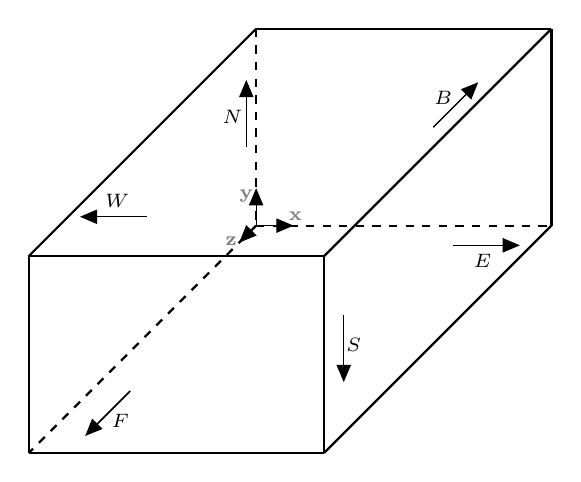
\begin{tikzpicture}[]
      \path pic[font=\scriptsize,scale=2.50]{geo};
    \end{tikzpicture}
  }
  \subfloat[]{
    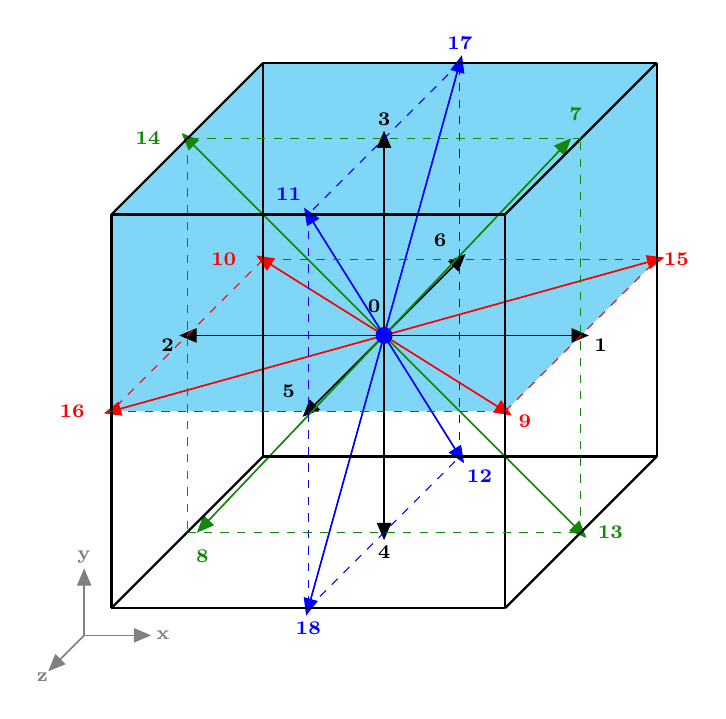
\begin{tikzpicture}[font=\scriptsize,scale=2.50,rotate around y=0,rotate around y=0]

      \fill[cyan!50] (-1,1,1) -- (0,1,1) -- (0,0,1) -- (-1,0,1) -- cycle; %  3.west-north-front
      \fill[cyan!50] (-1,1,1) -- (0,1,1) -- (0,1,0) -- (-1,1,0) -- cycle;
      \fill[cyan!50] (-1,1,1) -- (-1,1,0) -- (-1,0,0) -- (-1,0,1) -- cycle;
      \fill[cyan!50] (0,1,1) -- (0,1,0) -- (0,0,0) -- (0,0,1) -- cycle;
      \fill[cyan!50] (-1,0,1) -- (0,0,1) -- (0,0,0) -- (-1,0,0) -- cycle;
      \fill[cyan!50] (-1,1,0) -- (0,1,0) -- (0,0, 0) -- (-1,0,0) -- cycle;

      \fill[cyan!50] (1,1,1) -- (0,1,1) -- (0,0,1) -- (1,0,1) -- cycle; %  4.east-north-front
      \fill[cyan!50] (1,1,1) -- (0,1,1) -- (0,1,0) -- (1,1,0) -- cycle;
      \fill[cyan!50] (1,1,1) -- (1,1,0) -- (1,0,0) -- (1,0,1) -- cycle;
      \fill[cyan!50] (0,1,1) -- (0,1,0) -- (0,0,0) -- (0,0,1) -- cycle;
      \fill[cyan!50] (1,0,1) -- (0,0,1) -- (0,0,0) -- (1,0,0) -- cycle;
      \fill[cyan!50] (1,1,0) -- (0,1,0) -- (0,0, 0) -- (1,0,0) -- cycle;

      \fill[cyan!50] (-1,1,-1) -- (0,1,-1) -- (0,0,-1) -- (-1,0,-1) -- cycle; %  7.west-north-back
      \fill[cyan!50] (-1,1,-1) -- (0,1,-1) -- (0,1,0) -- (-1,1,0) -- cycle;
      \fill[cyan!50] (-1,1,-1) -- (-1,1,0) -- (-1,0,0) -- (-1,0,-1) -- cycle;
      \fill[cyan!50] (0,1,-1) -- (0,1,0) -- (0,0,0) -- (0,0,-1) -- cycle;
      \fill[cyan!50] (-1,0,-1) -- (0,0,-1) -- (0,0,0) -- (-1,0,0) -- cycle;
      \fill[cyan!50] (-1,1,0) -- (0,1,0) -- (0,0, 0) -- (-1,0,0) -- cycle;

      \fill[cyan!50] (1,1,-1) -- (0,1,-1) -- (0,0,-1) -- (1,0,-1) -- cycle; %  8. east-north-back
      \fill[cyan!50] (1,1,-1) -- (0,1,-1) -- (0,1,0) -- (1,1,0) -- cycle;
      \fill[cyan!50] (1,1,-1) -- (1,1,0) -- (1,0,0) -- (1,0,-1) -- cycle;
      \fill[cyan!50] (0,1,-1) -- (0,1,0) -- (0,0,0) -- (0,0,-1) -- cycle;
      \fill[cyan!50] (1,0,-1) -- (0,0,-1) -- (0,0,0) -- (1,0,0) -- cycle;
      \fill[cyan!50] (1,1,0) -- (0,1,0) -- (0,0, 0) -- (1,0,0) -- cycle;

      \path pic[font=\scriptsize,scale=2.50]{lat};
    \end{tikzpicture}
  }
  \caption{I=\{ 0,1,2,4,5,6,8,9,10,12,13,15,16,18\} and O=\{ 0,1,2,3,5,6,7,9,10,11,14,15,16,17\}}
\end{figure}

4. North
\begin{figure}[H]
  \centering

  \subfloat[]{
    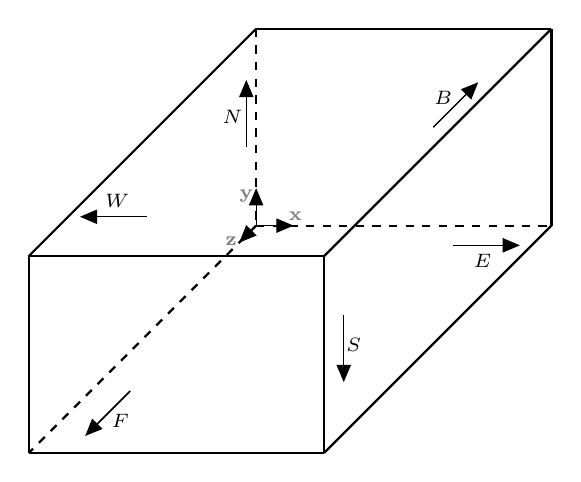
\begin{tikzpicture}[]
      \path pic[font=\scriptsize,scale=2.50]{geo};
    \end{tikzpicture}
  }
  \subfloat[]{
    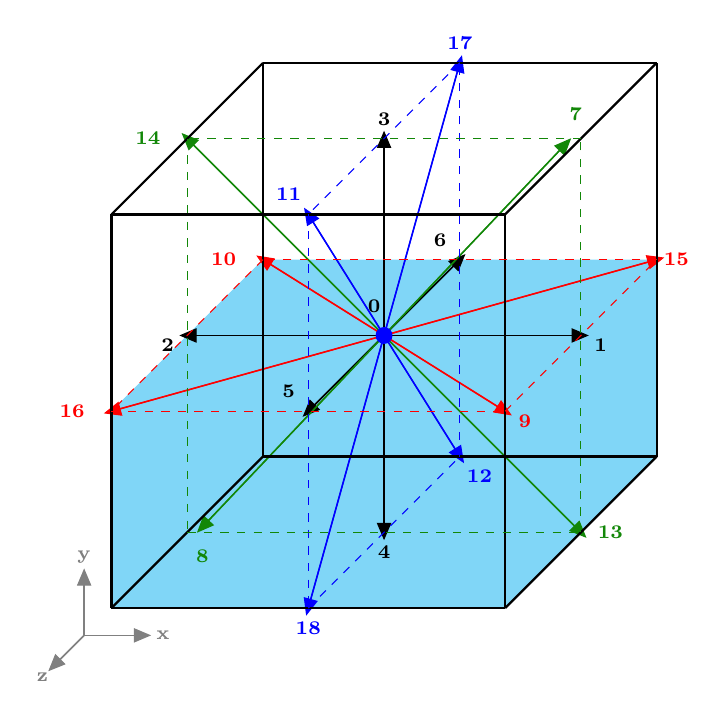
\begin{tikzpicture}[font=\scriptsize,scale=2.50,rotate around y=0,rotate around y=0]

      \fill[cyan!50] (-1,-1,1) -- (0,-1,1) -- (0,0,1) -- (-1,0,1) -- cycle; %  1.west-south-front
      \fill[cyan!50] (-1,-1,1) -- (0,-1,1) -- (0,-1,0) -- (-1,-1,0) -- cycle;
      \fill[cyan!50] (-1,-1,1) -- (-1,-1,0) -- (-1,0,0) -- (-1,0,1) -- cycle;
      \fill[cyan!50] (0,-1,1) -- (0,-1,0) -- (0,0,0) -- (0,0,1) -- cycle;
      \fill[cyan!50] (-1,0,1) -- (0,0,1) -- (0,0,0) -- (-1,0,0) -- cycle;
      \fill[cyan!50] (-1,-1,0) -- (0,-1,0) -- (0,0, 0) -- (-1,0,0) -- cycle;

      \fill[cyan!50] (0,-1,1) -- (1,-1,1) -- (1,0,1) -- (0,0,1) -- cycle;% 2. east-south-front
      \fill[cyan!50] (1,-1,1) -- (1,-1,0) -- (1,0,0) -- (1,0,1) -- cycle;
      \fill[cyan!50] (0,-1,1) -- (1,-1,1) -- (1,-1,0) -- (0,-1,0) -- cycle;
      \fill[cyan!50] (1,0,1) -- (0,0,1) -- (0,0,0) -- (1,0,0) -- cycle;
      \fill[cyan!50] (0,-1,0) -- (1,-1,0) -- (1,0, 0) -- (0,0,0) -- cycle;
      \fill[cyan!50] (0,-1,1) -- (0,-1,0) -- (0,0,0) -- (0,0,1) -- cycle;

      \fill[cyan!50] (-1,-1,-1) -- (0,-1,-1) -- (0,0,-1) -- (-1,0,-1) -- cycle; %  5. west-south-back
      \fill[cyan!50] (-1,-1,-1) -- (0,-1,-1) -- (0,-1,0) -- (-1,-1,0) -- cycle;
      \fill[cyan!50] (-1,-1,-1) -- (-1,-1,0) -- (-1,0,0) -- (-1,0,-1) -- cycle;
      \fill[cyan!50] (0,-1,-1) -- (0,-1,0) -- (0,0,0) -- (0,0,-1) -- cycle;
      \fill[cyan!50] (-1,0,-1) -- (0,0,-1) -- (0,0,0) -- (-1,0,0) -- cycle;
      \fill[cyan!50] (-1,-1,0) -- (0,-1,0) -- (0,0, 0) -- (-1,0,0) -- cycle;

      \fill[cyan!50] (1,-1,-1) -- (0,-1,-1) -- (0,0,-1) -- (1,0,-1) -- cycle; %  6.east-south-back
      \fill[cyan!50] (1,-1,-1) -- (0,-1,-1) -- (0,-1,0) -- (1,-1,0) -- cycle;
      \fill[cyan!50] (1,-1,-1) -- (1,-1,0) -- (1,0,0) -- (1,0,-1) -- cycle;
      \fill[cyan!50] (0,-1,-1) -- (0,-1,0) -- (0,0,0) -- (0,0,-1) -- cycle;
      \fill[cyan!50] (1,0,-1) -- (0,0,-1) -- (0,0,0) -- (1,0,0) -- cycle;
      \fill[cyan!50] (1,-1,0) -- (0,-1,0) -- (0,0, 0) -- (1,0,0) -- cycle;

      \path pic[font=\scriptsize,scale=2.50]{lat};
    \end{tikzpicture}
  }
  \caption{I=\{ 0,1,2,3,5,6,7,9,10,11,14,15,16,17\} and O=\{ 0,1,2,4,5,6,8,9,10,12,13,15,16,18\}}
\end{figure}

5. Back
\begin{figure}[H]
  \centering

  \subfloat[]{
    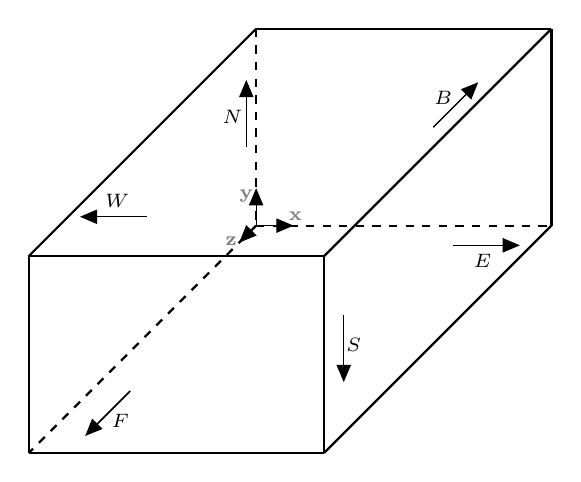
\begin{tikzpicture}[]
      \path pic[font=\scriptsize,scale=2.50]{geo};
    \end{tikzpicture}
  }
  \subfloat[]{
    \begin{tikzpicture}[font=\scriptsize,scale=2.50,rotate around y=0,rotate around y=0]

      \fill[cyan!50] (-1,-1,1) -- (0,-1,1) -- (0,0,1) -- (-1,0,1) -- cycle; %  1.west-south-front
      \fill[cyan!50] (-1,-1,1) -- (0,-1,1) -- (0,-1,0) -- (-1,-1,0) -- cycle;
      \fill[cyan!50] (-1,-1,1) -- (-1,-1,0) -- (-1,0,0) -- (-1,0,1) -- cycle;
      \fill[cyan!50] (0,-1,1) -- (0,-1,0) -- (0,0,0) -- (0,0,1) -- cycle;
      \fill[cyan!50] (-1,0,1) -- (0,0,1) -- (0,0,0) -- (-1,0,0) -- cycle;
      \fill[cyan!50] (-1,-1,0) -- (0,-1,0) -- (0,0, 0) -- (-1,0,0) -- cycle;

      \fill[cyan!50] (0,-1,1) -- (1,-1,1) -- (1,0,1) -- (0,0,1) -- cycle;% 2. east-south-front
      \fill[cyan!50] (1,-1,1) -- (1,-1,0) -- (1,0,0) -- (1,0,1) -- cycle;
      \fill[cyan!50] (0,-1,1) -- (1,-1,1) -- (1,-1,0) -- (0,-1,0) -- cycle;
      \fill[cyan!50] (1,0,1) -- (0,0,1) -- (0,0,0) -- (1,0,0) -- cycle;
      \fill[cyan!50] (0,-1,0) -- (1,-1,0) -- (1,0, 0) -- (0,0,0) -- cycle;
      \fill[cyan!50] (0,-1,1) -- (0,-1,0) -- (0,0,0) -- (0,0,1) -- cycle;

      \fill[cyan!50] (-1,1,1) -- (0,1,1) -- (0,0,1) -- (-1,0,1) -- cycle; %  3.west-north-front
      \fill[cyan!50] (-1,1,1) -- (0,1,1) -- (0,1,0) -- (-1,1,0) -- cycle;
      \fill[cyan!50] (-1,1,1) -- (-1,1,0) -- (-1,0,0) -- (-1,0,1) -- cycle;
      \fill[cyan!50] (0,1,1) -- (0,1,0) -- (0,0,0) -- (0,0,1) -- cycle;
      \fill[cyan!50] (-1,0,1) -- (0,0,1) -- (0,0,0) -- (-1,0,0) -- cycle;
      \fill[cyan!50] (-1,1,0) -- (0,1,0) -- (0,0, 0) -- (-1,0,0) -- cycle;

      \fill[cyan!50] (1,1,1) -- (0,1,1) -- (0,0,1) -- (1,0,1) -- cycle; %  4.east-north-front
      \fill[cyan!50] (1,1,1) -- (0,1,1) -- (0,1,0) -- (1,1,0) -- cycle;
      \fill[cyan!50] (1,1,1) -- (1,1,0) -- (1,0,0) -- (1,0,1) -- cycle;
      \fill[cyan!50] (0,1,1) -- (0,1,0) -- (0,0,0) -- (0,0,1) -- cycle;
      \fill[cyan!50] (1,0,1) -- (0,0,1) -- (0,0,0) -- (1,0,0) -- cycle;
      \fill[cyan!50] (1,1,0) -- (0,1,0) -- (0,0, 0) -- (1,0,0) -- cycle;

      \path pic[font=\scriptsize,scale=2.50]{lat};
    \end{tikzpicture}
  }
  \caption{I=\{ 0,1,2,3,4,6,7,8,10,12,13,14,15,17\} and O=\{ 0,1,2,3,4,5,7,8,9,11,13,14,16,18\}}
\end{figure}

6. Front
\begin{figure}[H]
  \centering

  \subfloat[]{
    \begin{tikzpicture}[]
      \path pic[font=\scriptsize,scale=2.50]{geo};
    \end{tikzpicture}
  }
  \subfloat[]{
    \begin{tikzpicture}[font=\scriptsize,scale=2.50,rotate around y=0,rotate around y=0]

      \fill[cyan!50] (-1,-1,-1) -- (0,-1,-1) -- (0,0,-1) -- (-1,0,-1) -- cycle; %  5. west-south-back
      \fill[cyan!50] (-1,-1,-1) -- (0,-1,-1) -- (0,-1,0) -- (-1,-1,0) -- cycle;
      \fill[cyan!50] (-1,-1,-1) -- (-1,-1,0) -- (-1,0,0) -- (-1,0,-1) -- cycle;
      \fill[cyan!50] (0,-1,-1) -- (0,-1,0) -- (0,0,0) -- (0,0,-1) -- cycle;
      \fill[cyan!50] (-1,0,-1) -- (0,0,-1) -- (0,0,0) -- (-1,0,0) -- cycle;
      \fill[cyan!50] (-1,-1,0) -- (0,-1,0) -- (0,0, 0) -- (-1,0,0) -- cycle;

      \fill[cyan!50] (1,-1,-1) -- (0,-1,-1) -- (0,0,-1) -- (1,0,-1) -- cycle; %  6.east-south-back
      \fill[cyan!50] (1,-1,-1) -- (0,-1,-1) -- (0,-1,0) -- (1,-1,0) -- cycle;
      \fill[cyan!50] (1,-1,-1) -- (1,-1,0) -- (1,0,0) -- (1,0,-1) -- cycle;
      \fill[cyan!50] (0,-1,-1) -- (0,-1,0) -- (0,0,0) -- (0,0,-1) -- cycle;
      \fill[cyan!50] (1,0,-1) -- (0,0,-1) -- (0,0,0) -- (1,0,0) -- cycle;
      \fill[cyan!50] (1,-1,0) -- (0,-1,0) -- (0,0, 0) -- (1,0,0) -- cycle;

      \fill[cyan!50] (-1,1,-1) -- (0,1,-1) -- (0,0,-1) -- (-1,0,-1) -- cycle; %  7.west-north-back
      \fill[cyan!50] (-1,1,-1) -- (0,1,-1) -- (0,1,0) -- (-1,1,0) -- cycle;
      \fill[cyan!50] (-1,1,-1) -- (-1,1,0) -- (-1,0,0) -- (-1,0,-1) -- cycle;
      \fill[cyan!50] (0,1,-1) -- (0,1,0) -- (0,0,0) -- (0,0,-1) -- cycle;
      \fill[cyan!50] (-1,0,-1) -- (0,0,-1) -- (0,0,0) -- (-1,0,0) -- cycle;
      \fill[cyan!50] (-1,1,0) -- (0,1,0) -- (0,0, 0) -- (-1,0,0) -- cycle;

      \fill[cyan!50] (1,1,-1) -- (0,1,-1) -- (0,0,-1) -- (1,0,-1) -- cycle; %  8. east-north-back
      \fill[cyan!50] (1,1,-1) -- (0,1,-1) -- (0,1,0) -- (1,1,0) -- cycle;
      \fill[cyan!50] (1,1,-1) -- (1,1,0) -- (1,0,0) -- (1,0,-1) -- cycle;
      \fill[cyan!50] (0,1,-1) -- (0,1,0) -- (0,0,0) -- (0,0,-1) -- cycle;
      \fill[cyan!50] (1,0,-1) -- (0,0,-1) -- (0,0,0) -- (1,0,0) -- cycle;
      \fill[cyan!50] (1,1,0) -- (0,1,0) -- (0,0, 0) -- (1,0,0) -- cycle;

      \path pic[font=\scriptsize,scale=2.50]{lat};
    \end{tikzpicture}
  }
  \caption{I=\{ 0,1,2,3,4,5,7,8,9,11,13,14,16,18\} and O=\{ 0,1,2,3,4,6,7,8,10,12,13,14,15,17\}}
\end{figure}

\end{document}

